%% abtex2-modelo-trabalho-academico.tex, v-1.6.1 laurocesar
%% Copyright 2012-2013 by abnTeX2 group at http://abntex2.googlecode.com/
%%
%% This work may be distributed and/or modified under the
%% conditions of the LaTeX Project Public License, either version 1.3
%% of this license or (at your option) any later version.
%% The latest version of this license is in
%%   http://www.latex-project.org/lppl.txt
%% and version 1.3 or later is part of all distributions of LaTeX
%% version 2005/12/01 or later.
%%
%% This work has the LPPL maintenance status `maintained'.
%%
%% The Current Maintainer of this work is the abnTeX2 team, led
%% by Lauro César Araujo. Further information are available on
%% http://abntex2.googlecode.com/
%%
%% This work consists of the files abntex2-modelo-trabalho-academico.tex,
%% abntex2-modelo-include-comandos and abntex2-modelo-references.bib
%%

% ------------------------------------------------------------------------
% ------------------------------------------------------------------------
% abnTeX2: Modelo de Trabalho Academico (tese de doutorado, dissertacao de
% mestrado e trabalhos monograficos em geral) em conformidade com
% ABNT NBR 14724:2011: Informacao e documentacao - Trabalhos academicos -
% Apresentacao
% ------------------------------------------------------------------------
% ------------------------------------------------------------------------

% verso e anverso:
\documentclass[12pt,openright,oneside,a4paper,english,brazil]{abntex2}

% apenas verso:
% \documentclass[12pt,oneside,a4paper,english,french,spanish,brazil]{abntex2}


% ---
% PACOTES
% ---

% ---
% Pacotes fundamentais
% ---
\usepackage{cmap}				% Mapear caracteres especiais no PDF
\usepackage{lmodern}			% Usa a fonte Latin Modern
\usepackage[T1]{fontenc}		% Selecao de codigos de fonte.
\usepackage[utf8]{inputenc}		% Codificacao do documento (conversão automática dos acentos)
\usepackage{lastpage}			% Usado pela Ficha catalográfica
\usepackage{indentfirst}		% Indenta o primeiro parágrafo de cada seção.
\usepackage[usenames,dvipsnames]{color}				% Controle das cores
\usepackage{graphicx}			% Inclusão de gráficos
\usepackage{multicol}			% enumerate com várias colunas
\usepackage{pdfpages}
\usepackage{tabularx}
\usepackage{xspace}
\usepackage{listings}
\usepackage{color}
%\usepackage{caption}
\usepackage{array}
\usepackage{courier}
\usepackage{amsmath}
\usepackage{multirow}

\definecolor{mygreen}{rgb}{0,0.6,0}
\definecolor{mygray}{rgb}{0.5,0.5,0.5}
\definecolor{mymauve}{rgb}{0.58,0,0.82}

\lstset{ %
  backgroundcolor=\color{white},   % choose the background color; you must add \usepackage{color} or \usepackage{xcolor}
  basicstyle=\footnotesize,        % the size of the fonts that are used for the code
  breakatwhitespace=false,         % sets if automatic breaks should only happen at whitespace
  breaklines=true,                 % sets automatic line breaking
  captionpos=b,                    % sets the caption-position to bottom
  commentstyle=\color{mygreen},    % comment style
  deletekeywords={...},            % if you want to delete keywords from the given language
  escapeinside={\%*}{*)},          % if you want to add LaTeX within your code
  extendedchars=true,              % lets you use non-ASCII characters; for 8-bits encodings only, does not work with UTF-8
  frame=single,                    % adds a frame around the code
  keepspaces=true,                 % keeps spaces in text, useful for keeping indentation of code (possibly needs columns=flexible)
  keywordstyle=\color{blue},       % keyword style
  language=Octave,                 % the language of the code
  morekeywords={*,...},            % if you want to add more keywords to the set
  numbers=left,                    % where to put the line-numbers; possible values are (none, left, right)
  numbersep=5pt,                   % how far the line-numbers are from the code
  numberstyle=\tiny\color{mygray}, % the style that is used for the line-numbers
  rulecolor=\color{black},         % if not set, the frame-color may be changed on line-breaks within not-black text (e.g. comments (green here))
  showspaces=false,                % show spaces everywhere adding particular underscores; it overrides 'showstringspaces'
  showstringspaces=false,          % underline spaces within strings only
  showtabs=false,                  % show tabs within strings adding particular underscores
  stepnumber=2,                    % the step between two line-numbers. If it's 1, each line will be numbered
  stringstyle=\color{mymauve},     % string literal style
  tabsize=2,                       % sets default tabsize to 2 spaces
  title=\lstname                   % show the filename of files included with \lstinputlisting; also try caption instead of title
}


% ---

% ---
% Pacotes de citações
% ---
%\usepackage[brazilian,hyperpageref]{backref}	 % Paginas com as citações na bibl
\usepackage[alf]{abntex2cite}	% Citações padrão ABNT

% ---
% CONFIGURAÇÕES DE PACOTES
% ---
% Configurações do pacote backref
% Usado sem a opção hyperpageref de backref
%\renewcommand{\backrefpagesname}{Citado na(s) página(s):~}
% Texto padrão antes do número das páginas
%\renewcommand{\backref}{}
% Define os textos da citação
%\renewcommand*{\backrefalt}[4]{
%	\ifcase #1 %
%		Nenhuma citação no texto.%
%	\or
%		Citado na página #2.%
%	\else
%		Citado #1 vezes nas páginas #2.%
%	\fi}%
% ---
\newcommand{\TODO}[1]{\textcolor{red}{\large TODO:} \textcolor{Purple}{[#1]~}}

%\DeclareCaptionFormat{reverse}{\hfill#3#2#1}
%\DeclareCaptionLabelFormat{fullparens}{(\bothIfFirst{#1}{˜}#2)}
%\DeclareCaptionLabelSeparator{fill}{\hfill}

\newcommand{\resumodocapitulo}{\section*{Resumo do Capítulo}}

\newcommand{\fontedaimg}[1]{%
%\captionsetup{%
        %font=footnotesize,%
        %justification=raggedright,%
        %singlelinecheck=false,%
        %format=reverse,%
        %font=it
%        justification=raggedleft, format={reverse},%
%font={small,it}
%}%
\ABNTEXfontereduzida{}Fonte: #1}

\newcommand{\fonteAP}{\fontedaimg{Autor}}

\newcolumntype{C}[1]{>{\centering\arraybackslash} m{#1} }


% Novo list of (listings) para QUADROS

\newcommand{\quadroname}{Quadro}
\newcommand{\listofquadrosname}{Lista de quadros}

\newfloat[chapter]{quadro}{loq}{\quadroname}
\newlistof{listofquadros}{loq}{\listofquadrosname}
\newlistentry{quadro}{loq}{0}

% configurações para atender às regras da ABNT
\counterwithout{quadro}{chapter}
\renewcommand{\cftquadroname}{\quadroname\space} 
\renewcommand*{\cftquadroaftersnum}{\hfill--\hfill}


% ---
% Informações de dados para CAPA e FOLHA DE ROSTO
% ---
\titulo{Realidade Virtual aplicada ao desenvolvimento de competências e habilidades de raciocínio lógico em crianças}
\autor{Gianfranco Pennacchi\\Vinícius Menézio\\}
% XXX WHY THE HELL THE LAST \\ INFLUENCES IN THE _PREVIOUS_ SPACING!!!
\local{São Paulo}

%% TODO XXX XXX XXX XXX XXX XXX XXX XXX XXX TODO
%% TODO                                     TODO
%% TODO  Nao esquecer de mudar a data aqui! TODO
%% TODO                                     TODO
%% TODO XXX XXX XXX XXX XXX XXX XXX XXX XXX TODO

\data{2016}
\orientador{Prof. Dr. Ricardo Nakamura}
\coorientador{Profa. Msc. Lucy Mari Tabuti}
%coorientador{Equipe \abnTeX}
%\instituicao{Área de Concentração Sistemas Digitais}
%  Universidade de São Paulo
%  \par
%  Escola Politécnica
%  \par
%  Departamento de Engenharia de Computação e Sistemas Digitais}

\tipotrabalho{Trabalho de Formatura}
% O preambulo deve conter o tipo do trabalho, o objetivo,
% o nome da instituição e a área de concentração
\preambulo{Trabalho de Formatura apresentado ao Departamento de Engenharia de Computação e Sistemas
Digitais da Escola Politécnica da Universidade de São Paulo para obtenção do Diploma de Engenheiro}
% ---


% ---
% Configurações de aparência do PDF final

% alterando o aspecto da cor azul
\definecolor{blue}{RGB}{41,5,195}

% informações do PDF
\makeatletter
\hypersetup{
     	%pagebackref=true,
		pdftitle={\@title},
		pdfauthor={\@author},
    	pdfsubject={\imprimirpreambulo},
	    pdfcreator={LaTeX with abnTeX2},
        pdfkeywords={keywords aqui},
		colorlinks=true,       		% false: boxed links; true: colored links
    	linkcolor=black,          	% color of internal links
    	citecolor=black,        		% color of links to bibliography
    	filecolor=black,      		% color of file links
		urlcolor=black,
		bookmarksdepth=4
}
\makeatother
% ---

% ---
% Espaçamentos entre linhas e parágrafos
% ---

% O tamanho do parágrafo é dado por:
\setlength{\parindent}{1.3cm}

% Controle do espaçamento entre um parágrafo e outro:
\setlength{\parskip}{0.2cm}  % tente também \onelineskip

% ---
% compila o indice
% ---
\makeindex
% ---

% ----
% Início do documento
% ----
\begin{document}

% Retira espaço extra obsoleto entre as frases.
\frenchspacing

% ----------------------------------------------------------
% ELEMENTOS PRÉ-TEXTUAIS
% ----------------------------------------------------------
% \pretextual

% ---
% Capa
% ---
\imprimircapa
% ---

\begin{comment}
\begin{folhadeaprovacao}

  \begin{center}
    {\ABNTEXchapterfont\large\imprimirautor}

    \vspace*{\fill}\vspace*{\fill}
    {\ABNTEXchapterfont\bfseries\Large\imprimirtitulo}
    \vspace*{\fill}

    \hspace{.45\textwidth}
    \begin{minipage}{.5\textwidth}
        \imprimirpreambulo
    \end{minipage}%
    \vspace*{\fill}
   \end{center}

   \imprimirlocal, X de dezembro de 2015:

   \assinatura{\textbf{\imprimirorientador} \\ Orientador}
   %\assinatura{\textbf{Professor} \\ Convidado 1}
   %\assinatura{\textbf{Professor} \\ Convidado 2}
   %\assinatura{\textbf{Professor} \\ Convidado 3}
   %\assinatura{\textbf{Professor} \\ Convidado 4}

   \begin{center}
    \vspace*{0.5cm}
    {\large\imprimirlocal}
    \par
    {\large\imprimirdata}
    \vspace*{1cm}
  \end{center}

\end{folhadeaprovacao}
\end{comment}

\begin{folhadeaprovacao}

  \begin{center}
    {\ABNTEXchapterfont\large\imprimirautor}

    \vspace*{\fill}\vspace*{\fill}
    {\ABNTEXchapterfont\bfseries\Large\imprimirtitulo}
    \vspace*{\fill}

    \hspace{.45\textwidth}
    \begin{minipage}{.5\textwidth}
        \imprimirpreambulo
    \end{minipage}%
    \vspace*{\fill}
   \end{center}

   \begin{center}
    \vspace*{0.5cm}
    {\large\imprimirlocal}
    \par
    {\large\imprimirdata}
    \vspace*{1cm}
  \end{center}

\end{folhadeaprovacao}
% ---
% Inserir a ficha bibliografica
% ---

% Isto é um exemplo de Ficha Catalográfica, ou ``Dados internacionais de
% catalogação-na-publicação''. Você pode utilizar este modelo como referência.
% Porém, provavelmente a biblioteca da sua universidade lhe fornecerá um PDF
% com a ficha catalográfica definitiva após a defesa do trabalho. Quando estiver
% com o documento, salve-o como PDF no diretório do seu projeto e substitua todo
% o conteúdo de implementação deste arquivo pelo comando abaixo:
%
\begin{fichacatalografica}
%    \includepdf{fig/fichaCatalografica.pdf}
\end{fichacatalografica}
%\begin{comment}
\begin{fichacatalografica}
	\vspace*{\fill}					% Posição vertical
	\hrule							% Linha horizontal
	\begin{center}					% Minipage Centralizado
	\begin{minipage}[c]{12.5cm}		% Largura

	\imprimirautor
	\hspace{0.5cm} \imprimirtitulo  / \imprimirautor. --
	\imprimirlocal, \imprimirdata-

	\hspace{0.5cm} \pageref{LastPage} p. : il. (algumas color.) ; 30 cm.

	\hspace{0.5cm} \imprimirorientadorRotulo~\imprimirorientador

	\hspace{0.5cm}
	\parbox[t]{\textwidth}{\imprimirtipotrabalho~--~\imprimirinstituicao,
	\imprimirdata.}

	\hspace{0.5cm}
                \TODO{Definir palavras chave com a biblioteca}

	\hspace{8.75cm} CDU 02:141:005.7

	\end{minipage}
	\end{center}
	\hrule
\end{fichacatalografica}
%\end{comment}
% ---

\begin{comment}
% ---
% Inserir errata
% ---
\begin{errata}
Elemento opcional da \citeonline[4.2.1.2]{NBR14724:2011}. Exemplo:

\vspace{\onelineskip}

FERRIGNO, C. R. A. \textbf{Tratamento de neoplasias ósseas apendiculares com
reimplantação de enxerto ósseo autólogo autoclavado associado ao plasma
rico em plaquetas}: estudo crítico na cirurgia de preservação de membro em
cães. 2011. 128 f. Tese (Livre-Docência) - Faculdade de Medicina Veterinária e
Zootecnia, Universidade de São Paulo, São Paulo, 2011.

\begin{table}[htb]
\center
\footnotesize
\begin{tabular}{|p{1.4cm}|p{1cm}|p{3cm}|p{3cm}|}
  \hline
   \textbf{Folha} & \textbf{Linha}  & \textbf{Onde se lê}  & \textbf{Leia-se}  \\
    \hline
    1 & 10 & auto-conclavo & autoconclavo\\
   \hline
\end{tabular}
\end{table}

\end{errata}
% ---

% ---
% Inserir folha de aprovação
% ---

% Isto é um exemplo de Folha de aprovação, elemento obrigatório da NBR
% 14724/2011 (seção 4.2.1.3). Você pode utilizar este modelo até a aprovação
% do trabalho. Após isso, substitua todo o conteúdo deste arquivo por uma
% imagem da página assinada pela banca com o comando abaixo:
%
% \includepdf{folhadeaprovacao_final.pdf}
%
\end{comment}

% ---
% Folha de rosto
% (o * indica que haverá a ficha bibliográfica)
% ---
\imprimirfolhaderosto*
% ---

% ---
\begin{comment}

% ---
% Dedicatória
% ---
\begin{dedicatoria}
   \vspace*{\fill}
   \centering
   \noindent
   \textit{ Este trabalho é dedicado às crianças adultas que,\\
   quando pequenas, sonharam em se tornar cientistas.} \vspace*{\fill}
\end{dedicatoria}
% ---

% ---
% Agradecimentos
% ---
\begin{agradecimentos}
Os agradecimentos principais são direcionados à Gerald Weber, Miguel Frasson,
Leslie H. Watter, Bruno Parente Lima, Flávio de Vasconcellos Corrêa, Otavio Real
Salvador, Renato Machnievscz\footnote{Os nomes dos integrantes do primeiro
projeto abn\TeX\ foram extraídos de
\url{http://codigolivre.org.br/projects/abntex/}} e todos aqueles que
contribuíram para que a produção de trabalhos acadêmicos conforme
as normas ABNT com \LaTeX\ fosse possível.

Agradecimentos especiais são direcionados ao Centro de Pesquisa em Arquitetura
da Informação\footnote{\url{http://www.cpai.unb.br/}} da Universidade de
Brasília (CPAI), ao grupo de usuários
\emph{latex-br}\footnote{\url{http://groups.google.com/group/latex-br}} e aos
novos voluntários do grupo
\emph{\abnTeX}\footnote{\url{http://groups.google.com/group/abntex2} e
\url{http://abntex2.googlecode.com/}}~que contribuíram e que ainda
contribuirão para a evolução do \abnTeX.

\end{agradecimentos}
% ---

% ---
% Epígrafe
% ---
\begin{epigrafe}
    \vspace*{\fill}
	\begin{flushright}
		\textit{``Não vos amoldeis às estruturas deste mundo, \\
		mas transformai-vos pela renovação da mente, \\
		a fim de distinguir qual é a vontade de Deus: \\
		o que é bom, o que Lhe é agradável, o que é perfeito.\\
		(Bíblia Sagrada, Romanos 12, 2)}
	\end{flushright}
\end{epigrafe}
% ---
\end{comment}

% ---
% RESUMOS
% ---
% resumo em português
\begin{resumo}
\begin{comment}
O resumo deve ser redigido, preferencialmente, na terceira pessoa do singular com verbo na voz ativa, em parágrafo único, e conter no máximo 500 palavras.
\end{comment}

O sucesso e a taxa de adoção de jogos eletrônicas na educação foi, 
até os dias atuais, insuficiente para encorajar a implementação 
em larga escala de experiências lúdicas como formas de facilitar 
o aprendizado.Isso decorre principalmente de três fatos: 
uma divergência entre os objetivos de design de jogos 
educacionais e os de jogos não-educacionais; dificuldades 
práticas de prover cada estudante com o hardware e o software 
necessários; e a necessidade de supervisão de professores 
para que os resultados desejados sejam alcançados.

Contudo, conforme a tecnologia móvel se aproxima de seu ponto 
de maturidade, e dispositivos de realidade virtual tecnologicamente 
viáveis e financeiramente acessíveis começam a adentrar o 
mercado em massa, um momento crítico se aproxima no qual 
experiências educativas verdadeiramente imersivas e cuidadosamente 
projetadas possam ser desenvolvidas, valendo-se de pouco mais 
do que os celulares que as crianças já carregam em seus bolsos.

O intuito deste projeto de Trabalho de Conclusão de Curso 
(TCC) é criar um jogo que, ao fazer uso de tecnologia móvel 
e de realidade virtual, possa providenciar um ambiente 
imersivo e fértil para a exploração e desenvolvimento de 
habilidades motoras, lógicas e do raciocínio espacial de 
crianças, expandindo a fronteira de conhecimento relacionada 
a jogos digitais aplicados à educação, alinhado ao projeto 
da doutoranda Lucy Mari Tabuti.

As tecnologias utilizadas são o \textit{Google Cardboard} para 
gerar a realidade virtual e o\textit{ Leap Motion} para a captura 
de gestos. O jogo foi desenvolvido na ferramenta \textit{Unity}, 
em virtude das facilidades propiciadas por ela, em 
especial lidando com ambientes tridimensionais.

 \vspace{\onelineskip}

 \noindent
 \textbf{Palavras-chaves}: Educação, imersão, realidade virtual, raciocínio lógico, jogo.
\end{resumo}
 
% resumo em inglês
\begin{resumo}[Abstract]
 \begin{otherlanguage*}{english}
   The success and adoption rate of video games in education 
   have, up to this day, not proven sufficient to encourage 
   large-scale implementation of gaming as a means to 
   supplement and facilitate learning. This stems from 
   both a divergence of the design goals when comparing 
   educational to non-educational digital games, as well 
   as from the practical difficulty of providing each student 
   with the necessary hardware, software and support from 
   teachers to ensure the desired results are being achieved 
   from the playing of the games.
   
   However, as mobile technology achieves its point of 
   maturity, and affordable, technically viable virtual 
   reality-capable devices start to enter the market en 
   masse, we stand at a critical moment in which truly 
   immersive, carefully designed learning experiences 
   can be developed, making use of little more than the 
   smartphones children already carry in their pockets.
   
   The purpose of this work is to develop a game that, 
   making use of mobile technology and virtual reality, 
   may provide a fertile and immersive environment for 
   exploration and development of motor, logic and spatial 
   reasoning skills, while expanding the frontiers of 
   educational gaming, aligned to the projects of 
   Professor Lucy Mari Tabuti.
   
   The technologies to be employed are the 
   Google Carboard virtual reality headset and the 
   Leap Motion hand gesture detector. The game will be 
   developed using the Unity engine, given its high level 
   capabilities and suitability to 3D environments.

    \vspace{\onelineskip}

    \noindent
    \textbf{Key-words}: Education, immersion, virtual reality, logic puzzle, logical reasoning.
  \end{otherlanguage*}
\end{resumo}

\begin{comment}
% resumo em francês
\begin{resumo}[Résumé]
 \begin{otherlanguage*}{french}
    Il s'agit d'un résumé en français.

   \vspace{\onelineskip}

   \noindent
   \textbf{Mots-clés}: latex. abntex. publication de textes.
 \end{otherlanguage*}
\end{resumo}

% resumo em espanhol
\begin{resumo}[Resumen]
 \begin{otherlanguage*}{spanish}
   Este es el resumen en español.

   \vspace{\onelineskip}

   \noindent
   \textbf{Palabras clave}: latex. abntex. publicación de textos.
 \end{otherlanguage*}
\end{resumo}
% ---
\end{comment}
 
% ---
% inserir lista de ilustrações
% ---
\pdfbookmark[0]{\listfigurename}{lof}
\listoffigures*
\cleardoublepage

% ---

% ---
% inserir lista de quadros
% ---
\pdfbookmark[0]{\listofquadrosname}{loq}
\listofquadros*
\cleardoublepage
% ---

% ---
% inserir lista de tabelas
% ---
\pdfbookmark[0]{\listtablename}{lot}
\listoftables*
\cleardoublepage

% ---

% ---
% inserir lista de abreviaturas e siglas
% ---
\begin{siglas}
	\item[ MEC ]			Ministerio da Educação
\item[ PCN ]            Parâmetros Curriculares Nacionais
\item[ GDD ]            Game Design Document
\item[ SDK ]            Software Development Kit


\end{siglas}
% ---

\begin{comment}
% ---
% inserir lista de símbolos
% ---
\begin{simbolos}
  \item[$ \Gamma $] Letra grega Gama
  \item[$ \Lambda $] Lambda
  \item[$ \zeta $] Letra grega minúscula zeta
  \item[$ \in $] Pertence
\end{simbolos}
% ---
\end{comment}

% ---
% inserir o sumario
% ---
\pdfbookmark[0]{\contentsname}{toc}
\tableofcontents*
\cleardoublepage
% ---

% ----------------------------------------------------------
% ELEMENTOS TEXTUAIS
% ----------------------------------------------------------
\textual

% ----------------------------------------------------------
% ----------------------------------------------------------
% Corpo do TCC (Em outro arquivo)
% ----------------------------------------------------------
% ----------------------------------------------------------
\graphicspath{ {images/} }

% ----------------------------------------------------------
% Introdução
% ----------------------------------------------------------
\chapter{Introdução}

O emprego de jogos digitais como ferramento de auxílio na educação é um conceito estudado há décadas. Tentativas de criar \textit{software} que tome proveito deste tipo de mídia para ensinar determinados tópicos ou fomentar o desenvolvimento de habilidades específicas em crianças existem desde ao menos a década de 1970, com a criação do Consórcio de Computação Educacional de Minnesotta, MECC, cujo objetivo era auxiliar escolas do estado de Minnesota, nos EUA, a integrar o uso de computadores ao ensino, de acordo com \cite{lussenhop:2016:oregon-trail}.

Além de prover infraestrutura e computadores às escolas locais, o MECC também incentivou a criação de inúmeros jogos educacionais. Um dos mais famosos destes foi o \textit{Oregon Trail}, criado por três professores, para ensinar aos alunos como era a vida dos colonos do século XIX nos EUA. 

Embora, de acordo com \cite{poli:2012:video-game-spore}, tenha sido demonstrado em alguns casos que o uso de jogos em sala de aula pode ser benéfica para o envolvimento e desempenho dos alunos, proporcionando um aumento de até 3 horas extras por semana de contato com o material da classe e até 5\% de notas mais altas, a utilização de jogos em sala de aula ainda é baixo, quase inexistente. Ainda de acordo com \cite{poli:2012:video-game-spore}, a principal causa disso é a dificuldade em manter o engajamento de alunos, a falta de conteúdo complementar e o orçamento limitado.

Considerando que a atividade de jogar videogames é a quarta atividade mais comum entre adolescentes no Brasil, como visto em \cite{bndes:2014:mapeamento}, com 35\% das crianças entre 9 e 16 anos jogando diariamente, 45\% jogando pelo menos uma vez por semana e 19\% jogando uma vez ao mes, não se pode negar o potencial deste meio quando ao seu poder de disseminação de conhecimento e cultura, de uma maneira similar àquela do peças, literatura e filmes.

Com o amadurecimento e ubiquidade da tecnologia móvel, com 75.2\% da população e 49.9\% das crianças entre 10 e 14 possuindo um celular no Brasil, segundo dados de \cite{IBGE:2015:PNAD_TIC_2013}, um estudo aprofundado sobre alternativas para os jogos educacionais 'tradicionais', que combinem tecnologia e conhecimento para criar uma solução imersiva e efetiva, é necessária.

...

Recentemente, o tópico do desenvolvimento de \textit{video games} educativos tem voltado a estar em pauta, sobretudo dada a grande revolução tecnológica que tem ocorrido no campo de mídias interativas: a criação de dispositivos de realidade virtual.

...


\section{Objetivos}\label{sec-objetivos}

A partir da realização deste projeto, pretende-se dar os primeiros passos rumo a criação de jogos efetivamente educacionais, capazes de manter o engajamento e interesse de estudantes, ao passo que ensinam sobre tópicos e habilidades relevantes para seu desenvolvimento intelectual e psicológico.

Também pretende-se chegar a uma solução final de baixo custo, que possa ser implementada em larga escala por escolas e instituições educacionais sem impactos orçamentários proibitivos.

\TODO{Faltam objetivos}


\section{Justificativa}\label{sec-justificativas}

De acordo com o \textit{Organisation for Economic Co-operation and Development} (OCDE), o Brasil está em 58\textsuperscript{o} lugar dentre os 65 países estudados, com uma nota média em matemática de 391 (sendo que a média é 494), como visto em \cite{OECD:2016:low_performing_students}. Por este motivo, acreditamos ser importante pensar em maneiras de encorajar os alunos a estimular seu raciocínio lógico, visto que isto está intrinsicamente ligada ao desempenho nas ciências exatas.

\TODO{Escrever. Não precisa ser um section, mas precisa estar claro , assim como a motivação}

\section{Resultados esperados}\label{sec-resultados-esperados}

\TODO{Escrever}

\section{Trabalhos relacionados}\label{sec-trabalhos-relacionados}

\cite{Tabuti:2010:analise} estudam diferentes interações humano-computador, 
focando em como elas ajudam, ou atrapalham, o aprendizado em ambientes 
digitais. O estudo foi feito com base no cubo de Rubik, tanto em sua 
forma física quando em várias formas digitais.

\cite{SBGames:2015:RVAM} desenvolveram um jogo digital em realidade 
virtual, motivados pela baixa performance de alunos em aulas de matemática. 
O foco do jogo é ajudar o jogador aprender e reter conceitos apresentados 
em aula, através do uso de ambientes tridimensionais e com o auxílio de 
personagens e mundo visualmente atraentes. O jogo consiste de um mundo 
aberto e uma personagem controlável. O objetivo do jogo é conseguir o 
maior número de moedas o mais rápido possível, enquanto desviando de 
inimigos. Quando o jogador coleta uma moeda, aparece uma tela com uma questão 
de múltipla escolha. Caso o jogador acerte a pergunta, recebe a moeda 
colecionada, caso contrário é teleportado para o início da fase. O jogo pode 
ser dividido em dois estados: Um estado de 'jogo', quando o jogador está 
caçando as moedas, e um estado de 'aprendizado', quando o jogador está 
respondendo uma questão.

\cite{Alves:2015:VR_Quimica} também desenvolveram um jogo em realidade 
virtual, mas focando no ensino de química. Os gráficos são muito mais 
realistas do que o exemplo anterior, refletindo o público alvo mais 
maduro. O jogador controla uma personagem que é uma antropomorfização 
de um átomo de hidrogênio que tem que explorar o mundo (que é baseado 
na tabela periódica). Cada área diferente do mapa contém elementos 
diferentes, que interagem com o jogador de maneiras únicas. O objetivo 
do jogo é auxiliar o ensino de reações químicas para crianças. Através 
da transformação dos elementos em personagens, os autores tinham como 
objetivo ajudar o jogador a entender a química através de metáforas, 
contrapondo o exemplo anterior, onde o jogo é dividido em estados.


% o \label{codigo} serve para podermos fazer referencias para algo numerado, 
% como capitulos, tabelas, figuras, etc. 
% Quando colocamos o comando \ref{codigo}. o compilador troca o \ref{codigo}
% pelo numero atribuido ao \label{}
% ex. \label{tabelaLegal}
%   A tabela \ref{tabelaLegal} mostra que...
% vai ser substituido por
%   A tabela 2 mostra que

\chapter{Teoria}\label{cap-teoria}

O desenvolvimento de um jogo educacional, que funcione como uma ferramenta de auxílio ao
aprendizado em sala de aula, deve envolver a consideração de diversos aspectos
pedagógicos, sociais e de \textit{game design}.

Em primeiro lugar, é necessário o estabelecimento de um vocabulário comum e bem
definido, delineando conceitos relevantes que possam ser empregado ao longo da 
formulação e desenvolvimento do projeto.

% ---
\section{Jogos Digitais}\label{sec-jogosdigitais}
% ---

Para \cite{correia:2009:digital_games_spore}, jogos digitais são aqueles aonde exista
interação humano-computador, com o uso da tecnologia, e desenvolvidos para serem 
jogados em computadores, consoles ou outros dispositivos tecnológicos.

Tais jogos podem ser utilizados para auxiliar a assimilação de informações, permitindo
o aprendizado através de estratégias de ensino diferentes daquelas exploradas em sala
de aula, conforme demonstrado por \cite{fernandes:2012:digital_education}. Isto 
ocorre, em parte, por incentivar o aprendizado através da prática de atividades.

\cite{correia:2009:digital_games_spore} comprovam que a utilização de jogos 
na área de educação é importante não só pela motivação de se jogar um jogo, 
mas também pelo aprendizado através da exploração que ocorre. O 
desenvolvimento de jogos educacionais, porém, ainda são um desafio, devido 
à dificuldade de se juntar dois conceitos que parecem, a primeira vista,
ser discordantes: 'Educação' e 'Jogo'.


\TODO{"Vale a pena colocar mais uns dois parágrafos"}

% ---
\section{Mecânicas, dinâmicas e estética}\label{sec-mecanica-dinamica-estetica}
% ---

Segundo \cite{hunicke:2004}, um jogo, digital ou não, pode ser analisado através de
sua decomposição entre três componentes principais: mecânicas, dinâmicas e estética.

Mecânicas são entendidas como as regras efetivas do jogo, compondo as liberdades
concedidas e restrições impostas ao jogador, bem como seus objetivos, condições de
vitória e derrota. As mecânicas são a porção do jogo sobre a qual o desenvolvedor tem
controle direto, e influenciam a percepção das demais porções por parte do jogador.

Chama-se de dinâmicas os comportamentos emergentes demonstrados por jogadores em 
função das mecânicas. Encompassam desde comportamentos simples, como a reação de um
jogador a obstáculos do cenário, até a sofisticadas estratégias a respeito de quando
cooperar ou competir em jogos multi-jogador.

Estéticas definem a experiência essencial que o jogador tem ao longo de uma sessão de
jogo. Diz respeito às respostas emocionais, ao envolvimento e à imersão do jogador no
mundo virtual criado pelo desenvolvedor, e é útil para categorizar o jogo quanto às
sensações que ele é capaz de invocar.


% ---
\section{Realidade Virtual}\label{sec-realidadevirtual}
% ---

A Realidade Virtual é, de acordo com \cite{kirner:2007:RV_e_RA}, uma interface de
usuário avançada, que permite que o usuário veja, mova e interaja, em tempo real, 
om um ambiente tridimensional, através de dispositivos especiais. Em geral, a visão
tende a ser priorizada em interfaces de realidade virtual, mas a audição e o toque 
são também partes muito importantes da experiência do usuário.

Para \cite{kirner:2011:evolucao_RV}, um mundo virtual visto através de uma tela é
considerado não-imersiva, enquanto a percepção deste mundo virtual através de salas 
com multiprojeção ou por meio de capacetes é considerado imersivo. Desta forma, a
realidade virtual:

\begin{alineas}
	\item considera a entrada e saída feita com equipamentos capazes de manipular 
	informação multisensorial em tempo real;
	\item prioriza interação em tempo real sobre a qualidade das informações;
	\item requer processamento gráfico, háptico e sonoro em alta escala;
	\item leva em consideração que ações ocorrem em um espaço tridimensional;
	\item considera que equipamentos especiais para a interação multisensorial sejam
	utilizados;
	\item entende que o usuário necessita de um período de adaptação para entender a
	representação virtual do mundo.
\end{alineas}

% ---
\section{Competências e Habilidades do Raciocínio Lógico}\label{sec-competenciashabilidades}
% ---

O Ministério da Educação (MEC) define um conjunto de parâmetros que devem estar
presentes no currículo de escolas em todo o Brasil. Estes são os Parâmetros
Curriculares Nacionais (PCN), e abordam várias diferentes áreas importantes. 

As competências e habilidades de raciocínio lógico consideradas para análise
consistem de um subconjunto dos PCN, em especial, daqueles relativos ao 
raciocínio lógico, e são apresentados no \autoref{tabela:PCN}, retirado de
\cite{Tabuti:2015:tabela_habilidades}.

\renewcommand{\arraystretch}{1.2}
\begin{quadro}[ht] \scriptsize
	\centering
	\caption[Competências e habilidades]{Competências e habilidades relacionadas ao raciocínio lógico.}
	\begin{tabular} {| >{\centering\arraybackslash} m{2cm} | >{\centering\arraybackslash} m{1.5cm} | m{7cm} |}
		\hline
		Competência & Habilidade & \multicolumn{1}{>{\centering\arraybackslash}p{7cm} |}{Descrição da habilidade} \\
		\hline
		\multirow{1}[12]{*}{Análise} & H1 & Habilidade em resolver um problema complexo dividindo-o em subproblemas mais simples, com soluções mais imediatas \\ \cline{2-3}
		& H2 & Habilidade da recomposição dos resultados gerados para a solução do problema mais complexo \\
		\hline
		\multirow{1}[40]{*}{Síntese} & H3 & Habilidade em juntar informações e dados de um problema que sejam de diferentes naturezas \\ \cline{2-3}
		& H4 & Habilidade em avaliar a deficiência dessas informações para determinar a solução\\ \cline{2-3}
		& H5 & Habilidade em descobrir a falta de outras informações necessárias para a resolução do problema  \\ \cline{2-3}
		& H6 & Habilidade em priorizar essas informações para o desenvolvimento até atingir a solução \\ \cline{2-3}
		& H7 & Habilidade em ordenar essas informações de forma a obter uma sequência de desenvolvimento até atingir a solução \\
		\hline
		\multirow{1}[28]{*}{Inferência} & H8 & Habilidade em descobrir padrões em um conjunto de informações \\ \cline{2-3}
		& H9 & Habilidade em aplicar novamente determinada informação de forma a agregar novas informações a estrutura de padrões existente \\ \cline{2-3}
		& H10 & Habilidade em aplicar novamente determinada informação de forma a agregar novas informações num conjunto que preserve a estrutura de padrões existente \\ 
		\hline
	\end{tabular}

	\legend{\fontedaimg{\cite{Tabuti:2015:tabela_habilidades}}}
	\label{tabela:PCN}
\end{quadro}

As três competências demonstradas na tabela são importantes para a resolução 
de problemas. O desenvolvimento da competência de análise permite a resolução
de problemas através da divisão em problemas menores que tenham soluções 
mais simples, assim como a recomposição dos resultados gerados para solucionar 
o problema mais complexo. O desenvolvimento da competência de síntese permite
combinar e ordenar diferentes informações obtidas, afim de chegar a uma solução
geral. O desenvolvimento da competência de inferência, por sua vez, permite
reutilizar informações, padrões e relações aprendidas em situações anteriores 
para solucionar problemas futuros.

Dentro do escopo deste projeto, pretende-se dar maior enfoque na exploração e
desenvolvimento das habilidades H1, H2, H6 e H7.

\TODO{Explicar porque H1, H2, H6 e H7}

% ---
\section{Público alvo}\label{sec-publico-alvo}
% ---

Uma vez estipulado que o foco do projeto seria na criação de um jogo que
auxiliasse no aprendizado e retenção de habilidades do raciocínio lógico,
e que este jogo seria criado para uma plataforma de realidade virtual,
foi necessário refinar cuidadosamente a escolha de público alvo de modo a
garantir que jogadores estivessem dentro de uma faixa etária para a qual 
experiências de realidade virtual fossem manejáveis, e para a qual a
aprendizagem de habilidades de raciocínio lógico fosse tão benéfica quanto
possível.

\subsection{Adaptabilidade à realidade virtual}

Uma consideração a ser feita foi a capacidade de crianças mais novas de
compreender e interagir com dispositivos de realidade virtual.

Enquanto muitos dos dispositivos encontrados no mercado atualmente sugerem
limites mínimos para a idade de seus usuários na faixa dos 12 e 13 anos de
idade \cite{seeto:2016:playstation-vr}, o pesquisador da Universidade da Califórnia Martin Banks afirma que
não existem comprovações de malefícios específicos a crianças advindos do
uso de equipamentos de realidade virtual, e que quaisquer efeitos adversos
que venham a incorrer sobre crianças novas fazendo uso destes equipamentos
seriam "os mesmos que aqueles sofridos por adultos" \cite{hill:2016:vr-safe}.

Banks publicou também em 2008 um artigo \cite{hoffman2008vergence} detalhando como \textit{displays}
tridimensionais e, por extensão, \textit{headsets} de realidade virtual,
não acarretariam nos malefícios causados por "\textit{near work}" - ou
seja, atividades de leitura ou foco visual em páginas e \textit{displays}
muito próximos ao rosto -, uma vez que este tipo de \textit{display} gera
pontos focais virtuais a uma distância confortável dos olhos, muito além
da distância do \textit{display} em si.

Apesar de não haver um limite rígido para a idade mínima para interação com
realidade virtual, como será necessário que as crianças consigam compreender
e interagir com ambientes tridimensionais, estipulou-se 8 anos de idade como
o mínimo necessário para fazer uso do jogo desenvolvido, pois a partir desta
idade pode-se considerar completo o domínio da criança sobre suas habilidades
motoras, segundo o \textit{Children’s Therapy \& Family Resource Centre} \cite{ctfrc:motor-skills}.

\subsection{Desenvolvimento do raciocínio lógico}

...

Com estas questões em mente, pretendeu-se então projetar um jogo voltado para
alunos do ensino fundamental, entre 8 a 12 anos, numa faixa etária suficiente
para interagir com as tecnologias empregadas e essencial para a formação de
suas capacidades de raciocínio lógico.

% ---
\section{Tecnologia}\label{sec-tecnologia}
% ---

Para se desenvolver este projeto, foi necessário se familiarizar com algumas tecnologias, apresentadas a seguir. 
% ---
\subsection{Protocolo WebSocket}\label{subsec-teo-websocket}
% ---

O WebSocket é um protocolo de comunicação full-duplex que pode ser implementado
sobre uma conexão TCP, e foi padronizado em 2011 conforme descrito no RFC 6455
\cite{RFC:2011:websocket}. Ele foi desenvolvido para ser implementado em 
navegadores e servidores web, com o intuito de ampliar as possibilidades de
interação entre um navegador e um servidor. O protocolo permite que ambos os 
lados enviem mensagens ao outro a qualquer momento, sem a necessidade de um 
lado solicitar a mensagem. Mesmo tendo sido desenvolvido para uso em navegadores, 
o protocolo pode ser utilizado por qualquer aplicação de cliente e servidor.

Outro termo bastante relacionado ao WebSocket é o conceito de 
\textit{Push Notifications}, que são as mensagens enviadas de um servidor para 
um aplicativo executando em um celular para notificar o usuário de algum evento. 
O interessante é que o aplicativo não precisa ficar consultando o servidor 
(ex. \textit{polling}) para conseguir receber a mensagem, pois esta é enviada 
ao cliente quando o servidor quiser.

% ---
\subsection{Controlador Leap Motion}\label{subsec-teo-leap-motion}
% ---

O controlador \textit{Leap Motion}, da empresa de mesmo nome, começou a ser desenvolvido 
em 2008, contou com várias rodadas de investimento, e a primeira versão do 
\textit{Software Development Kit}(\textit{SDK}) foi lançada em maio de 2012. Dois anos depois, foi 
apresentada a segunda versão do \textit{SDK}, que melhorou bastante o rastreamento das 
mãos, e que é atualmente a versão mais utilizada. No início de 2016, a mais 
nova versão, chamada \textit{Orion}, foi lançada, desenvolvida especialmente para a 
realidade virtual, de acordo com \cite{leap:2016:changeset}

Para utilizar o controlador, são necessários 3 elementos diferentes: O hardware 
do controlador em si; um software rodando como um serviço em um computador; 
e um software 'cliente' que receberá os dados do serviço para utilizá-los, 
como pode ser visto na arquitetura do \textit{Leap Motion} \cite{leap:2016:architecture}

O controlador nada mais é do que um conjunto de duas câmeras e 3 LEDs, todos 
infravermelhos, de acordo com \cite{leap:2016:how-it-works}. Os LEDs projetam
luz infravermelha, que é refletida pelas mãos do usuário e captadas 
pelas câmeras. Estas imagens são enviadas ao serviço, 
que utiliza algoritmos de visão computacional para gerar modelos tridimensionais 
das mãos do usuário. A versão 2 do software aumentou muito a precisão do 
controlador por começar a trabalhar com um modelo esqueletal da mão, baseado 
na anatomia humana, ou seja, um modelo composto por 5 dedos, cada um contendo 
4 ossos. Este método insere restrições ao modelo, eliminando poses e movimentos 
que não seriam fisicamente possíveis.

O software cliente, então, pode receber os dados do serviço por duas interfaces:
Conversando diretamente com o serviço, utilizando uma biblioteca que acompanha o software, 
ou acessando o servidor \textit{WebSocket} que o serviço roda localmente.

A versão mais recente do \textit{SDK} ainda é nova, e tem focado na otimização dos 
algoritmos utilizados em várias áreas, tanto no processamento de imagens quanto 
outros algoritmos de 'suporte', como a detecção da adição ou remoção de um 
controlador. Visto a sua orientação para a realidade virtual, uma otimização 
importante foi em relação à mãos ocluídas, que sumiam em versões anteriores, 
conforme descrito em \cite{leap:2016:changeset}. É possível que comece a focar 
em coisas mais específicas para a realidade virtual em pouco tempo.

% ---
\subsection{Reconhecimento de Gestos}\label{subsubsec-teo-gestos}
% ---

\begin{figure}[h]
	\centering
	\caption{Modelo baseado na anatomia humana utilizado pelo controlador \textit{Leap Motion}}
	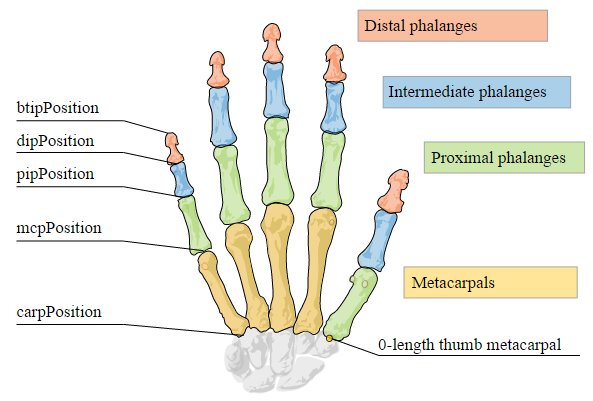
\includegraphics[width=0.7\textwidth]{leap-anatomical-hand}
	\legend{\fontedaimg{\cite{leap:2016:intro-skeletal}}}
	\label{fig:leap-anatomical-hand}
\end{figure}

Conforme mencionado na \autoref{subsec-teo-leap-motion}, a versão 
v2 em diante do controlador \textit{Leap Motion} utiliza um modelo 
da mão baseado na anatomia humana, conforme descrito 
em \cite{leap:2016:intro-skeletal}, e que pode ser visto 
na \autoref{fig:leap-anatomical-hand}. Isto significa que o 
rastreamento das mãos e dedos ficou mais preciso, pois a 
imagem capturada pelo controlador é processada e encaixada em 
um modelo anatomicamente correto. Desta forma, qualquer mão 
capturada terá 5 dedos, composto do número certo de ossos, e 
em posições e rotações anatomicamente possível. Isto também 
melhorou a oclusão de dedos, que antes sumiam do modelo da 
versão um(pois o modelo não teria necessariamente 5 dedos), 
agora podem ser estimados a partir do resto da mão.

A segunda versão do \textit{SDK} do \textit{Leap Motion} 
tinha, nativamente, o conceito de 'gestos', e o próprio 
\textit{SDK} disponibilizava alguns métodos para checar 
se alguns gestos básicos havia sido executado. Eram quatro 
o número de gestos reconhecidos: fazer um círculo com o 
dedo, deslizar o dedo, 'pressionar' um botão e tocar a 
tela, conforme descrito em \cite{leap:2016:gestures}. A 
versão \textit{Orion}, porém, no momento em que se 
iniciou o desenvolvimento deste trabalho, ainda não 
contava com a detecção automática de gestos, sendo 
necessário que o grupo desenvolvesse o código que o fizesse.

Dados os modelos das mãos, é possível detectar gestos através 
da posicão, rotação e velocidade da palma da mão, dos dedos, 
ou dos ossos individuais. Para a detecção de um dedo 
esticado, por exemplo, pode-se checar se o ângulo entre 
cada par de ossos adjacentes daquele dedo é \textit{pequeno} 
(aonde \textit{pequeno} deve ser definido com testes). 
Para se detectar uma palma virada para cima, pode-se 
verificar o vetor normal da palma (que nos é dada pelo 
\textit{SDK} do controlador) e ver se seu componente em 
y é positivo (tomando y como o eixo perpendicular ao 
plano do solo). Uma palma aberta apontando para cima, 
portando, pode ser detectada com o conjunto da detecção 
de um dedo esticado e da palma virada para cima.

É importante também notar que um mesmo gesto ou posicionamento
da mão pode ser descrita de várias formas. No caso do dedo esticado, 
por exemplo, poderia-se checar apenas o ângulo entre o primeiro e 
último ossos. Poderia, também, se calcular a distância entre estes
dois ossos. Dependendo do caso, as formas diferentes podem ser 
equivalentes, mas também podem apenas parecer iguais, mas quando
testados em ambientes diferentes, resultarão em saídas diferentes.
Por exemplo, uma mão menor poderia não ter o dedo considerado esticado
caso se utilizasse a distância entre os ossos.

Mais recentemente, porém, a empresa do \textit{Leap Motion} 
lançou módulos (chamados de \textit{utilities} no site) 
que permitem a detecção de gestos simples, não sendo 
mais necessário desenvolver código que o faça.

% ---
\subsection{Google Cardboard}\label{subsec-teo-google-cardboard}
% ---

O \textit{Google Cardboard} é um projeto da empresa Google criada em 2014 para 
fomentar o desenvolvimento de aplicações de realidade virtual. É composta por um 
\textit{headset} e de um software compatível. A ideia principal do projeto era
conseguir proporcionar a experiência de realidade virtual da forma mais barata 
o possível, conforme dito em \cite{cnet:2016:google-cardboard}. Para 
alcançar tal objetivo, o \textit{headset} é feito de papelão, 
de tal forma que o único subcomponente mais caro seja as lentes. Adicionalmente, 
um celular é utilizado tanto como poder de processamento do \textit{headset} 
quanto como a tela deste. Visto que uma grande parcela da população ja tem um 
\textit{smartphone}, estas partes do \textit{Cardboard} vêm de graça.

Quanto ao software compatível, é necessário que este divida a sua saída de 
vídeo (que será mostrado na tela do celular) em metades, uma para cada olho. 
Visto que cada imagem emula a visão de um olho, é necessário que as imagens 
venham de pontos de origem separados por uma distância equivalente àquela entre 
as duas pupilas, valor que varia entre 58 mm e 70 mm, de acordo com
\cite{dodgson:2004:svariation}. Adicionalmente, devido à distorção causada 
pelas lentes, é necessário que o software aplique a distorção inversa na imagem, 
de forma que a imagem após passar pela lente fique correta. É também necessário 
ler sensores encontrados no dispositivo móvel, como acelerômetros e giroscópios, 
e disponibilizar estes dados para que se possa implementar o movimento do 
usuário dentro do jogo ou aplicativo.

O \textit{SDK} do \textit{Google Cardboard}, distribuído pela própria Google e disponível online 
em \cite{google:2016:cardboardSDK}, já faz todas estas transformações necessárias 
na imagem, além de enviar os dados de movimento, ja processados, de volta ao
software que esteja utilizando o \textit{SDK}.


% o \label{codigo} serve para podermos fazer referencias para algo numerado, 
% como capitulos, tabelas, figuras, etc. 
% Quando colocamos o comando \ref{codigo}. o compilador troca o \ref{codigo}
% pelo numero atribuido ao \label{}
% ex. \label{tabelaLegal}
%   A tabela \ref{tabelaLegal} mostra que...
% vai ser substituido por
%   A tabela 2 mostra que

\chapter{Metodologia}\label{cap-metodologia}

A metodologia empregada na realização deste projeto foi o processo iterativo 
de design do Ciclo Formal \cite{schell:2010:art_game_design}, um método que 
alia conceitos de desenvolvimento ágil advindos da engenharia de software com 
noções modernas de game design. A adoção desta metodologia se deu pelo seu 
enfoque em frequentes testes e rápida iteração sobre o projeto, processos
imprescindíveis no desenvolvimento de um jogo que atenda aos critérios 
educacionais estabelecidos, no limitado escopo estipulado.

No contexto deste projeto, a aplicação do Ciclo Formal pode ser descrita nos 
termos de duas etapas principais: formulação do problema e implementação iterativa.

% ---
\section{Formulação do problema}\label{sec-met-formulacao-problema}
% ---

Na etapa inicial de criação do projeto, é necessário enunciar cuidadosamente 
a problema a ser resolvido, levando em consideração os objetivos do jogo, 
sua demografia e o contexto em que ele será jogado. Também é necessário analisar 
os recursos disponíveis e o prazo para a criação do produto final, afim de 
definir um escopo claro para o projeto. A partir do levantamento dessas 
informações, têm-se os parâmetros a serem usados nas próximas etapas de criação 
do projeto.

Este problema é documentado na forma de um \textit{Game Design Document} (GDD), 
que servirá tanto como um relatório quanto como um ponto de referência para 
a realização do projeto nas etapas seguintes.

% ---
\section{Implementação iterativa}\label{sec-met-implementacao-iterativa}
% ---

\begin{figure}[!htb]
	\centering
	\caption{Ciclo de Boehm.}
	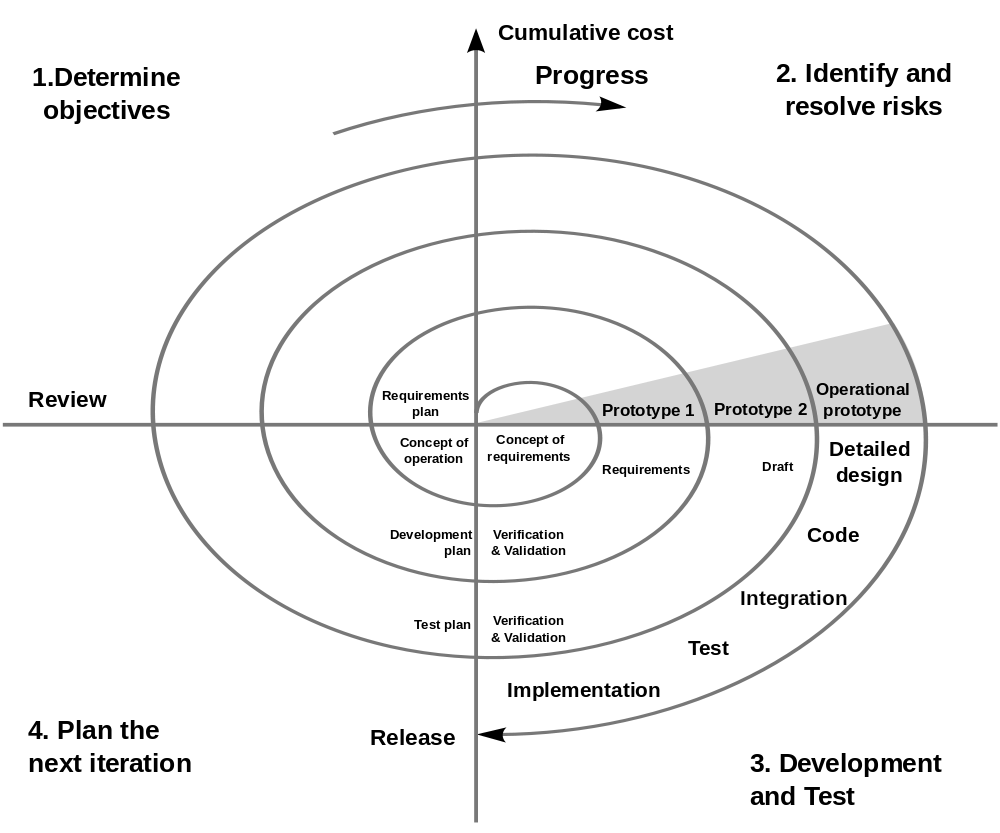
\includegraphics[width=0.5\textwidth]{ciclo_boehm}
	\legend{\fontedaimg{\cite{schell:2010:art_game_design}}}
	\label{fig:ciclo-boehm}
\end{figure}

Para a implementação do jogo em si, adota-se a metodologia de design iterativo,
consistente de uma aplicação do ciclo de desenvolvimento de software de 
Boehm (\autoref{fig:ciclo-boehm}) no âmbito de projetos de jogos digitais.

Nos termos dessa metodologia, um jogo digital deve ser implementado por meio de 
um processo iterativo, ciclando entre seis fase principais: \textit{Brainstorming}, 
escolha da solução, análise de riscos, prototipação, teste e análise e 
refinamento do \textit{design}.

% ---
\subsection{\textit{Brainstorming}}\label{subsec-met-brainstorming}
% ---

Nesta fase são propostas diversas potenciais soluções para o problema enunciado, 
com um enfoque na geração rápida do maior número possível de ideias, sendo 
evitado levantar críticas. As propostas são então listadas para avaliação quanto 
a seus méritos e adequação frente ao problema original elaborado, dentre as 
quais uma será eleita como o conceito do jogo, aprofundada e descrita formalmente 
em maiores detalhes.

\subsection{Escolha da solução}\label{subsec-met-escolha-solucao}

Uma das soluções propostas é escolhida, de acordo com sua aderência ao 
problema enunciado e viabilidade técnica. Sua descrição é então adicionada ao 
GDD, detalhando as características mecânicas, estéticas e tecnológicas. 
Esta descrição deverá ser tomada como referência para a implementação do jogo, 
e alterada conforme necessário durante as fases seguinte.

\subsection{Análise de riscos}\label{subsec-met-analise-riscos}

Durante a análise de riscos, um elemento específico do design deve ser 
considerado. Os potenciais riscos e dificuldades de implementação associados 
a esse segmento devem então ser levantados e listados, considerando as dinâmicas 
que pretende-se que esse elemento gere, sua aderência aos objetivos estipulados 
e eventuais problemas técnicos advindos de seu desenvolvimento.

\subsection{Prototipação}\label{subsec-met-prototipacao}

Nesta fase, procura-se elaborar rapidamente um protótipo que funcione como prova 
de conceito para o elemento recortado na fase anterior, de forma a eliminar ou 
mitigar os riscos observados. A ênfase deve ser na velocidade de implementação 
do protótipo, não em seu polimento ou reusabilidade dos recursos gerados em 
etapas posteriores do projeto.

\subsection{Teste}\label{subsec-met-teste}

Na fase de testes, o protótipo construído é avaliado quanto aos riscos 
delimitados na fase 3. A abrangência dos testes, variará de acordo com a natureza 
do elemento sendo testado e o atual estado de desenvolvimento do projeto como 
um todo, sendo que em testes realizados em projetos em etapas mais avançadas de 
seu desenvolvimento pedirão maior envolvimento de parcelas representativas 
do público alvo do produto final.

A adequação do elemento considerado aos objetivos esperados e sua eficácia 
na resolução dos problemas levantados determinarão o rumo das demais iterações 
do processo.

\subsection{Análise e refinamento do design}\label{subsec-met-analise-refinamento}

Durante esta fase, uma análise das fases anteriores deve ser feita, 
procurando-se ressaltar os motivos que levaram a eventuais inadequações do 
protótipo executado aos riscos previamente delimitados. Com base nos 
resultados observados, as modificações necessárias são feitas ao GDD, uma 
nova descrição do problema é redigida, e retorna-se à fase 1 para a construção 
de um novo protótipo com um maior grau de polimento.

Seguindo este método, o jogo toma forma gradativamente, através de iterações 
e prototipações sucessivas e aditivas, até que sua implementação esteja de 
acordo com o estado atual do GDD, e todos os objetivos definidos tenham 
sido atingidos.


% o \label{codigo} serve para podermos fazer referencias para algo numerado, 
% como capitulos, tabelas, figuras, etc. 
% Quando colocamos o comando \ref{codigo}. o compilador troca o \ref{codigo}
% pelo numero atribuido ao \label{}
% ex. \label{tabelaLegal}
%   A tabela \ref{tabelaLegal} mostra que...
% vai ser substituido por
%   A tabela 2 mostra que

\chapter{Fundamentação Teórica}\label{cap-fundamentacao}

Os conceitos teóricos explorados no planejamento e implementação deste projeto 
advém de diversas áreas do conhecimento - técnicas, antropológicas, 
pedagógicas, dentre outras - que foram empregadas conjuntamente para a 
obtenção do resultado desejado. Em termos gerais, pode-se dividir as 
disciplinas exploradas dentre três categorias principais:

\begin{itemize}[label={--},noitemsep,topsep=0pt,leftmargin=4mm]
	\item Conceituação pedagógica
	\item Exploração tecnológica
	\item \textit{Game design}
\end{itemize}
 
% ---
\section{Conceituação Pedagógica}\label{sec-fund-conceituacao-pedagogica}
% ---

Uma vez que a preocupação primária do trabalho é a elaboração de um produto 
que possa auxiliar educadores no ensino de \[...\]

\TODO{O capítulo todo}

% o \label{codigo} serve para podermos fazer referencias para algo numerado, 
% como capitulos, tabelas, figuras, etc. 
% Quando colocamos o comando \ref{codigo}. o compilador troca o \ref{codigo}
% pelo numero atribuido ao \label{}
% ex. \label{tabelaLegal}
%   A tabela \ref{tabelaLegal} mostra que...
% vai ser substituido por
%   A tabela 2 mostra que

\chapter{Desenvolvimento}\label{cap-desenvolvimento}

Segundo o processo iterativo de desenvolvimento descrito na metodologia, 
este projeto evoluiu ao longo de várias etapas de crescente complexidade.


% ---
\section{Objetivo e formulação do problema}\label{sec-objetivos-formulacao-problema}
% ---

Foi inicialmente elaborada uma enunciação geral do problema a ser resolvido: 
a criação de um jogo digital que, valendo-se de técnicas de realidade 
virtual, oferecesse uma experiência imersiva e educativa a crianças de 8 a 12 
anos de idade, de acordo com o recorte selecionado descrito no \autoref{cap-teoria}.
Tendo essa enunciação como base, pôde-se decidir a respeito de restrições, e 
do escopo que guiariam as etapas seguintes de conceituação do projeto.

% ---
\subsection{Delimitação do escopo}\label{subsec-delimitacao-escopo}
% ---
TODO

% ---
\subsection{Recorte do público alvo}\label{subsec-recorte-publico-alvo}
% ---

Em primeiro lugar, optou-se por restringir os equipamentos e tecnologias a 
serem empregados, de modo a facilitar a acessibilidade e adoção em sala de aula 
e diminuir os custos de implantação, sem que a experiência desejada tivesse de 
ser sacrificada. Isso levou à escolha do uso do \textit{Google Cardboard} 
como dispositivo principal de realidade virtual, por seu baixo custo comparado 
a demais alternativas de mercado, e sua integração a dispositivos móveis que, 
em muitos casos, já estariam ao alcance dos alunos, ou poderiam ser 
providenciados sem um grande impacto orçamentário.

Em adição ao \textit{Cardboard}, optou-se pela implementação do dispositivo 
detector de gestos manuais \textit{Leap Motion} como forma de \textit{input}
principal para o jogo, com a vantagem de ser uma alternativa de custo 
aceitável, capaz de providenciar uma experiência bastante direta na interação 
do aluno com o mundo do jogo, uma vez que permite que movimentos do jogador no 
mundo real sejam traduzidos em ações do mundo virtual, permitindo abstrair os 
dispositivos de entrada e saída por completo, e mantendo a imersão e engajamento.

Por fim, como restrição adicional, a ferramenta \textit{Unity} foi escolhida 
como \textit{engine} de desenvolvimento do jogo, por sua fácil integração 
ao hardware escolhido, e seu paradigma de desenvolvimento em mais alto nível do 
que as demais alternativas disponíveis, o que permitiria ao grupo focar-se 
na conceituação e implementação do jogo em si, sem prender-se a eventuais 
problemas relativos à configuração e uso do hardware, criação de APIs próprias 
ou preocupações com elementos mais elementares da criação de um jogo digital.
\TODO{Ultimos dois paragrafos não dizem a respeito ao publico alvo..}

% ---
\section{\textit{Brainstorming} e Seleção do Conceito do Jogo}\label{sec-brainstorming-conceito}
% ---

Com a enunciação do problema e as restrições de implementação bem definidas 
e acordadas pelo grupo, pôde-se passar para a etapa seguinte do desenvolvimento, 
o \textit{brainstorm}, durante o qual várias ideias foram debatidas e 
exploradas pelos membros do grupo. Nesta fase, diversas propostas foram feitas 
para uma solução que fizesse um bom uso dos recursos de realidade 
virtual disponíveis e gerasse um projeto adequado ao público alvo 
selecionado, resultando em um jogo intuitivo e divertido que fosse 
capaz de transmitir os conceitos lógicos e cognitivos relevantes.

As ideias geradas variaram desde jogos de um ritmo mais acelerado, no qual 
um jogador teria que categorizar elementos abstratos o mais rápido que 
pudesse - segundo características como cor, formato e tamanho - até experiências 
nas quais pressões de tempo e condições de falha estavam completamente 
ausentes, como jogos de resolução de quebra-cabeças tridimensionais, 
e são apresentadas a seguir.

% ---
\subsection{Ideias do Brainstorm}\label{subsec-ideias-brainstorm}
% ---

Na \autoref{fig:rascunhos-brainstorm} é possível ver o rascunho das ideias feitas durante o \textit{brainstorm}. 

\begin{figure}[h]
	\centering
	\caption{Primeiro rascunho do jogo}
	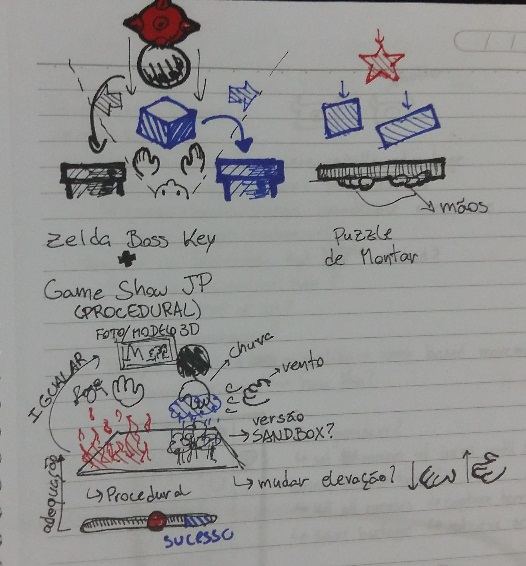
\includegraphics[width=0.5\textwidth]{first_concepts}
	\legend{\fonteAP}
	\label{fig:rascunhos-brainstorm}
\end{figure}

No canto superior direito, vê-se o rascunho de um conceito de jogo aonde 
peças vão caindo lentamente e devem ser empilhadas em uma bandeja ou 
superfície controlada pelo movimento das mãos do jogador, que deve 
movimentar a bandeja de forma que as peças que caem fiquem bem dispostas, 
em vez de tombar para fora da bandeja. Outra possibilidade é que as 
peças caindo tenham que se juntar para fazer um formato específico, 
ou até mesmo uma adaptação do famoso jogo \textit{Tetris}, mas 
tridimensional, aonde deve-se criar um plano inteiro sobre a bandeja 
(ao invés de uma linha, como no jogo original).

No canto superior esquerdo, existe o rascunho para um jogo de classificação. Assim como antes, peças vão caindo, e o jogador deve categorizar estas peças em uma de duas ou mais categorias, através de movimentos das mãos. No exemplo desenhado, o objetivo poderia ser mover todos os cubos azuis para a direita, esferas pretas para a esquerda, e não agir sobre as esferas com espinhos vermelhas. Outras variações poderiam ser feitas, também, como todos os cubos (independente de sua cor) vão para a direita, por exemplo. Existem inúmeras possibilidades, tendo como pré-requisito ser possível categorias os elementos. Adicionalmente, os exemplos dados foram com formas geométricas, mas podem ser abstraídas para quase qualquer área, como por exemplo elementos (ex. Separe os elementos que reajam com oxigênio), geografia (ex. Categorize os países por continente), história (ex. Classifique estes eventos como causas ou consequências da segunda guerra mundial), ou qualquer outro assunto que se consiga imaginar.

Logo abaixo do rascunho no canto superior esquerdo, estão as frases "Zelda Boss Key" e "Game Show JP". Estas são referências para uma terceira ideia de jogo, aonde é apresentado ao jogador uma peça tridimensional e uma abertura ou ranhura tridimensional. O jogador deve então, com movimentos da mão, rotacionar ou modificar a peça para que esta encaixe na ranhura/abertura. Dois exemplos da referência do jogo \textit{Legend of Zelda: Skyward Sword} podem ser vistas na \autoref{fig:zelda-key-puzzle}, aonde é possivel ver a peça na frente e, ao fundo, o encaixe.

\begin{figure}[h]
	\centering
	\caption{Dois exemplos do \textit{minigame} "Zelda Boss Key" do jogo \textit{Legend of Zelda: Skyward Sword}}
	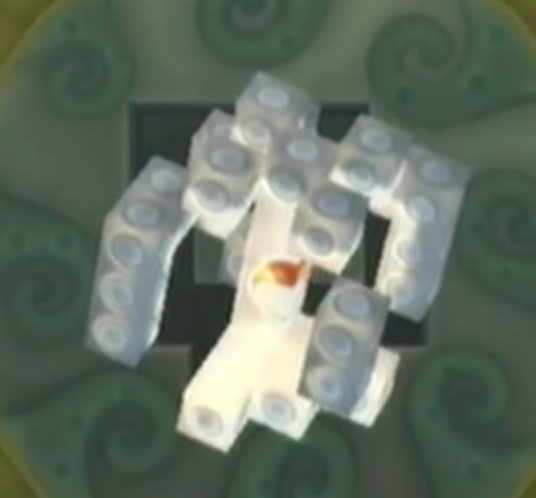
\includegraphics[width=0.3\textwidth]{zelda-puzzle-1}
	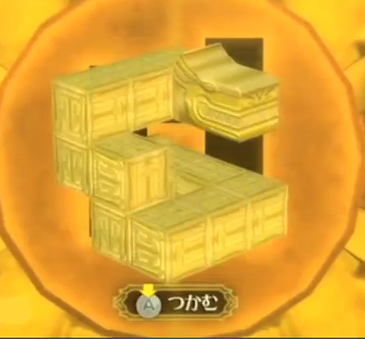
\includegraphics[width=0.3\textwidth]{zelda-puzzle-2}
	\legend{\fontedaimg{\cite{youtube:2016:boss-key}(esquerda) e \cite{zeldainformer:2016:boss-key}(direita)}}
	\label{fig:zelda-key-puzzle}
\end{figure}

Por último, na \autoref{fig:rascunhos-brainstorm}, no canto inferior esquerdo,
é possível ver o rascunho da quarta e última ideia. Neste jogo, os 
jogadores deparariam-se com um terreno digital composto por acidentes
geográficos como planaltos, depressões, corpos d'água e formações magmáticas, 
e poderiam modificá-lo a partir de gestos manuais simples que controlassem 
a elevação, precipitação, movimentação do ar, entre outros. O objetivo do jogo
é manipular a pequena configuração geológica tridimensional, de forma a chegar 
a um determinado estado pré-definido. O terreno seria subdivido em unidades 
cúbicas que poderiam ser manipuladas individualmente, fornecendo uma 
resolução suficiente para que configurações diversas e interessantes pudessem 
ser construídas, mas sem exigir uma precisão incompatível com os dispositivos 
de entrada e saída escolhidos.

% ---
\subsection{Seleção do Conceito do Jogo}\label{subsec-selecao-conceito}
% ---

Por fim, uma análise cuidadosa das limitações das tecnologias escolhidas, aliada 
a uma preocupação em manter o jogo intuitivo e imersivo levaram o grupo a 
escolher o último conceito dentre os quatro. Os dois primeiros conceitos, por 
mais interessante que fossem, tinham uma dependência muito forte sobre a
entrada do controlador \textit{Leap Motion}. Dado que o controlador não 
é completamente preciso e que poderia falhar em detectar movimentos ou 
capturar a mão do jogador, não queríamos que o jogador fosse punido por conta 
disso. Visto que os dois primeiros conceitos dependiam dos objetos caindo, 
uma falha do controlador poderia fazê-los perder, causando frustração. 
Entre o terceiro e quarto conceito, o grupo escolheu o último, devido a 
um interesse maior e também por ter um número muito maior de 
possibilidades. O jogador possivelmente perderia o interesse no terceiro 
conceito após poucas partidas do jogo.

Desta forma, o quarto conceito foi o escolhido para ser desenvolvido. O próximo passo era definir formalmente as mecânicas do jogo, assim como os elementos que o jogador poderia manipular. Estes elementos estão listados no \autoref{quadro:elementos}, junto das interações planejadas para cada um.

\begin{quadro}[htb] 
	\centering
	\caption[Elementos manipuláveis pelo jogador]{Elementos manipuláveis pelo jogador}
	
	\begin{tabular} {| >{\centering\arraybackslash} m{3cm} | >{\centering\arraybackslash} m{9cm} |}
		\hline
		\textbf{Elemento} & \textbf{Interação planejada} \\
		\hline
		Terra/Pedra & O principal elemento do mundo. O jogador consegue manipular os blocos de terra modificando sua altura, criando pilares ou buracos \\
		\hline
		Água & O jogador consegue causar precipitação em uma área pre-determinada, criando corpos d'água, como lagos \\
		\hline
		Fogo & O jogador pode colocar fogo em uma área pre-determinada, secando corpos d'água que estiverem ali \\
		\hline
		Vento & O jogador consegue criar correntezas de vento em uma das quatro direções cardeais. Se aplicados em uma configuração específica dos blocos, o vento cria ondas num corpo d'água que erode um bloco de terra/pedra, criando areia \\
		\hline
		Lava & Esse elemento não pode ser gerado pelo jogador, sendo encontrado no nível mais baixo do mundo em algumas fases. Se um buraco é escavado até este nível mais baixo, a lava começa a subir. Em contato com água, a lava vira terra/pedra \\
		\hline
		Areia & Criado pela erosão de terra/pedra devido à interação do vento com a água \\
		\hline
	\end{tabular}
	
	\legend{\fonteAP}
	\label{quadro:elementos}
\end{quadro}

Para que o jogo não fosse curto demais, foram então imaginados cenários 
que extrapolassem os usos básicos das 
mecânicas propostas, de maneiras que se alinhassem aos conceitos pedagógicos 
que deveriam ser transmitidos pelo jogo: desafios que dependessem da execução 
de tarefas em uma determinada ordem, em combinação com outras tarefas paralelas, 
ou dentro de um determinado limite de tempo. Nestes cenários, era esperado 
que jogadores conseguissem imaginar soluções mais sofisticadas, indo além 
das interações básicas às quais teriam acesso direto. Seria necessário 
movimentar massas de ar para jogar água contra blocos de terra (cujo rascunho 
é mostrado na \autoref{fig:rascunhos-praia}), formando 
praias; escavar o solo para alcançar câmaras magmáticos e formar vulcões; ou 
alterar o curso de corpos d'água para formar cascatas.

\begin{figure}[htb]
	\centering
	\caption{Rascunho de como criar uma praia, utilizando os elementos terra, água e ar}
	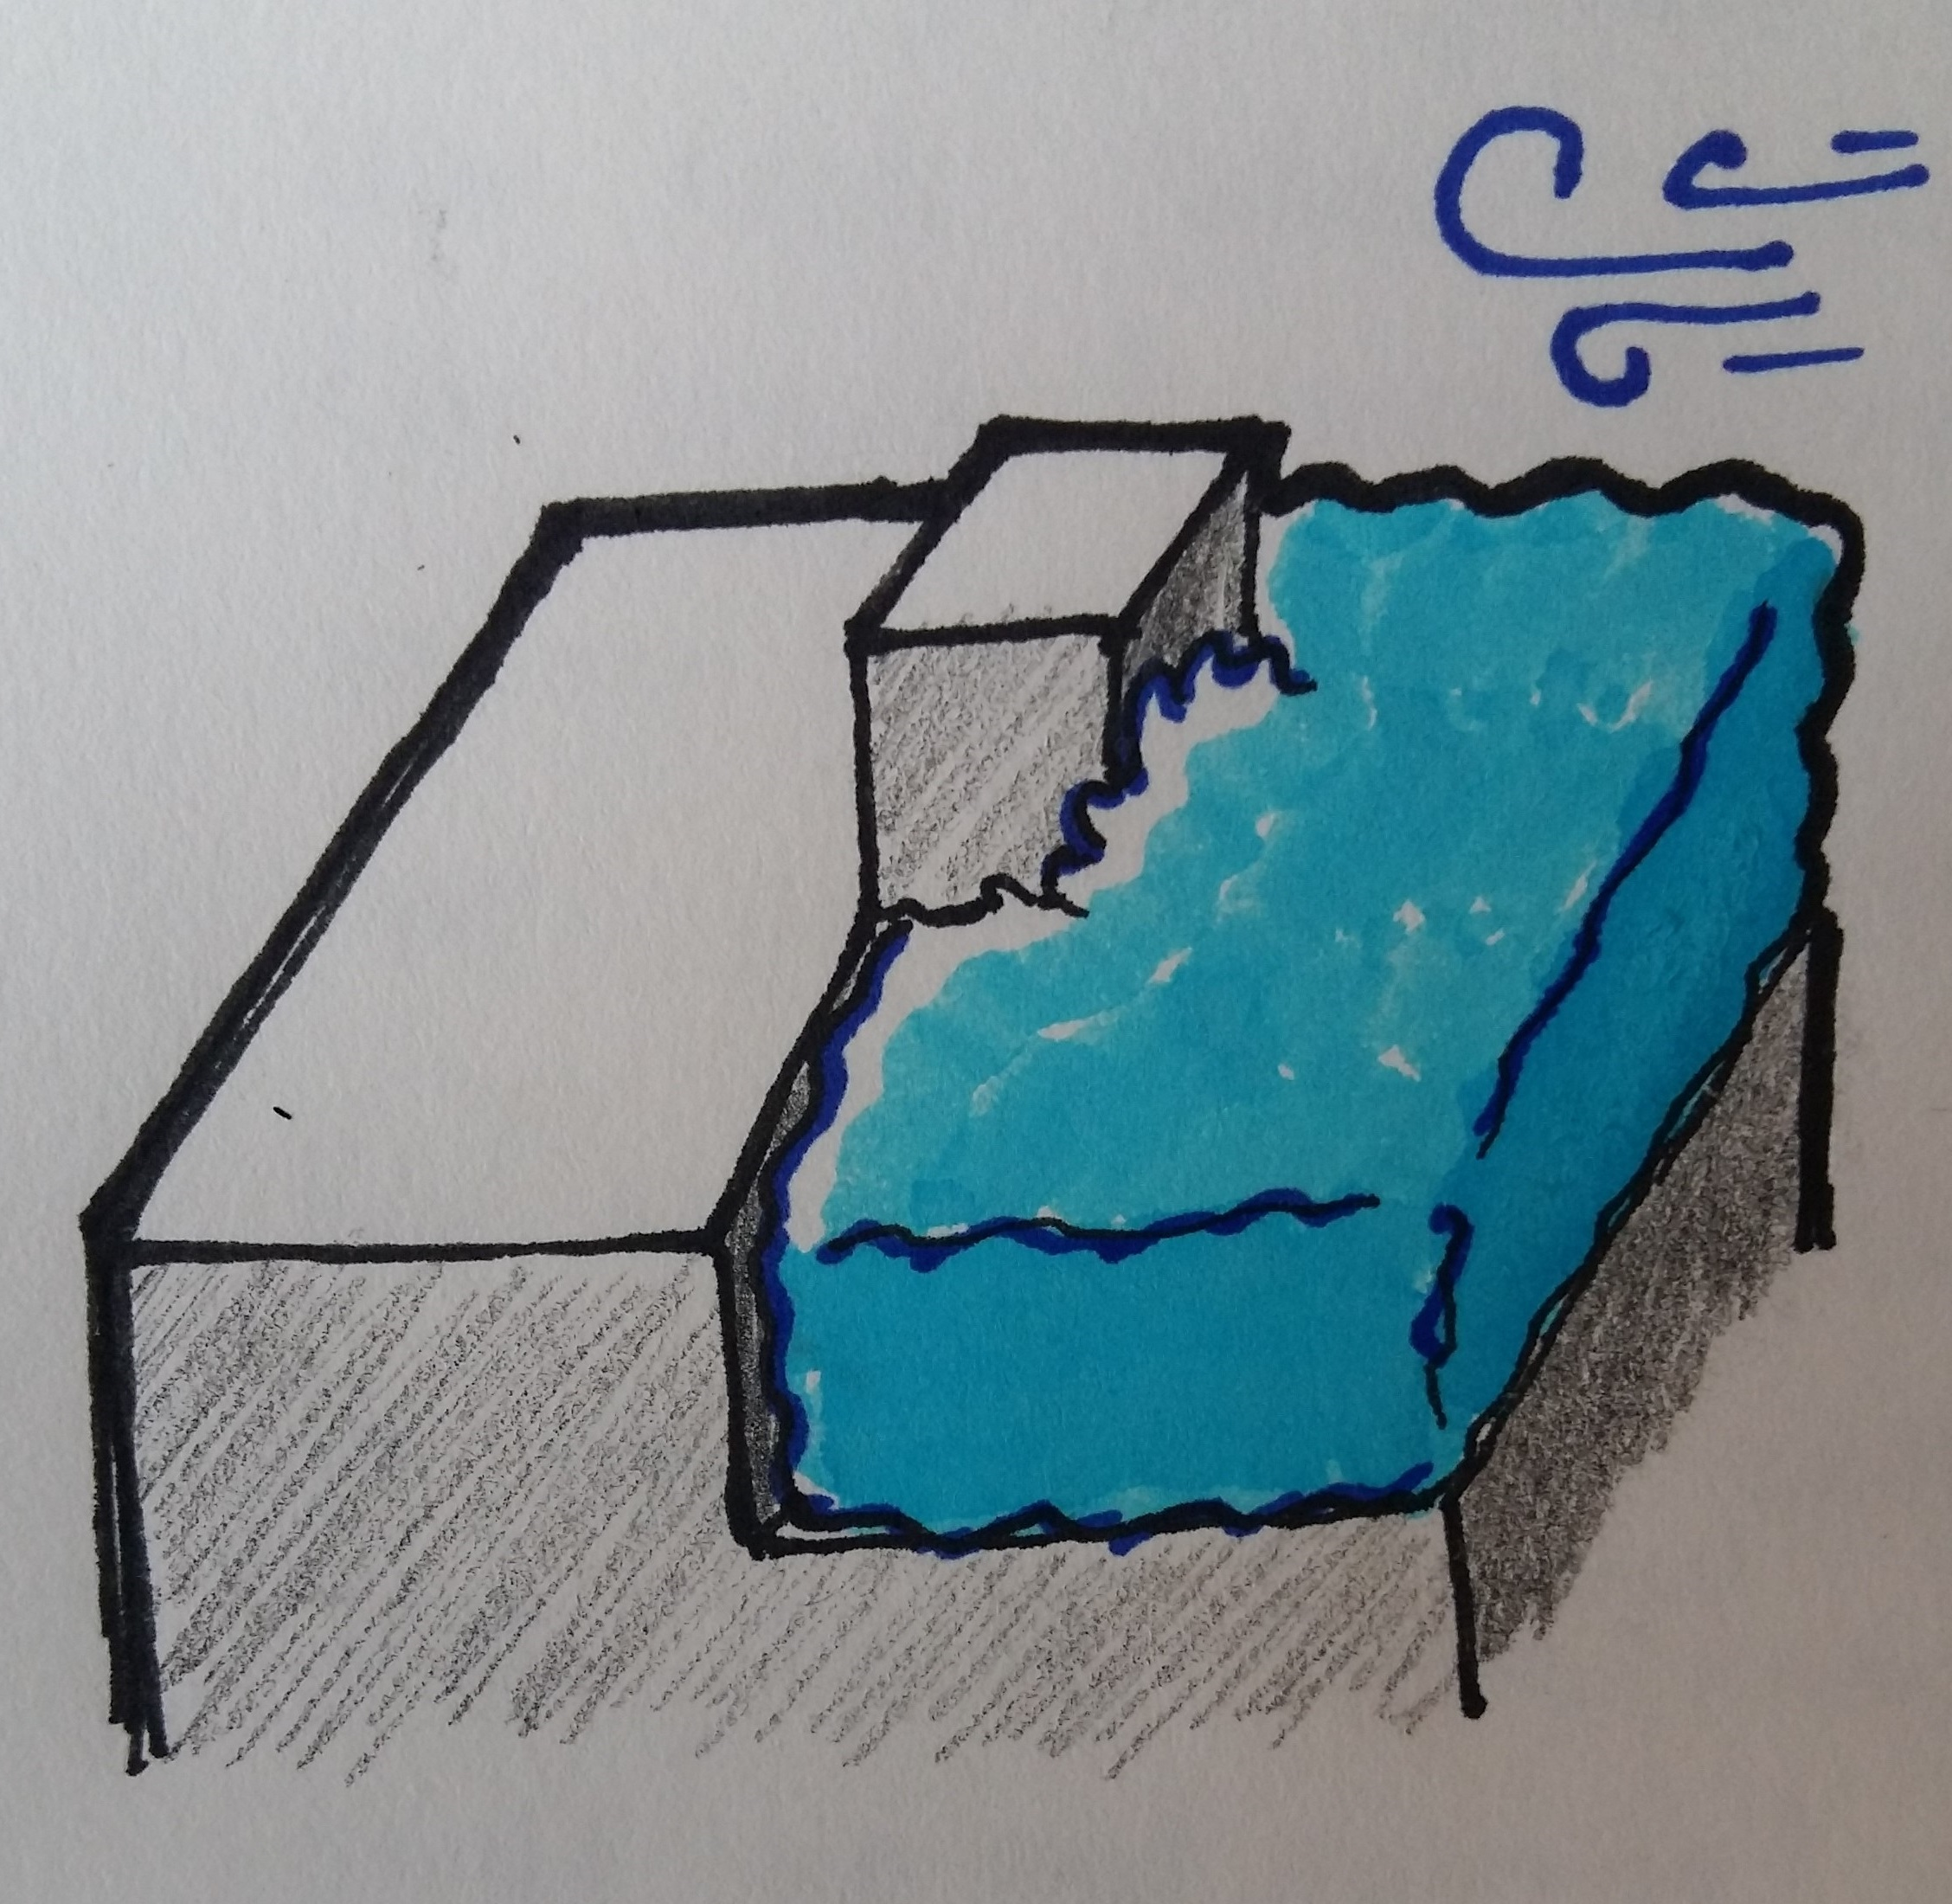
\includegraphics[width=0.5\textwidth]{draft2}
	\legend{\fonteAP}
	\label{fig:rascunhos-praia}
\end{figure}

Algumas primeiras ideias de possíveis fases também foram discutidas, para 
dar uma direção para a criação da prova de conceito. A primeira fase lidaria 
apenas com a mudança da elevação da terra e o jogador teria que criar um 
buraco e uma torre de terra, algo similar à \autoref{fig:rascunho-torre-buraco}.
Desta forma, a primeira prova de conceito já teria uma base 'jogável' 
para se testar a viabilidade do conceito.

\begin{figure}[h]
	\centering
	\caption{Rascunho de uma possível primeira fase}
	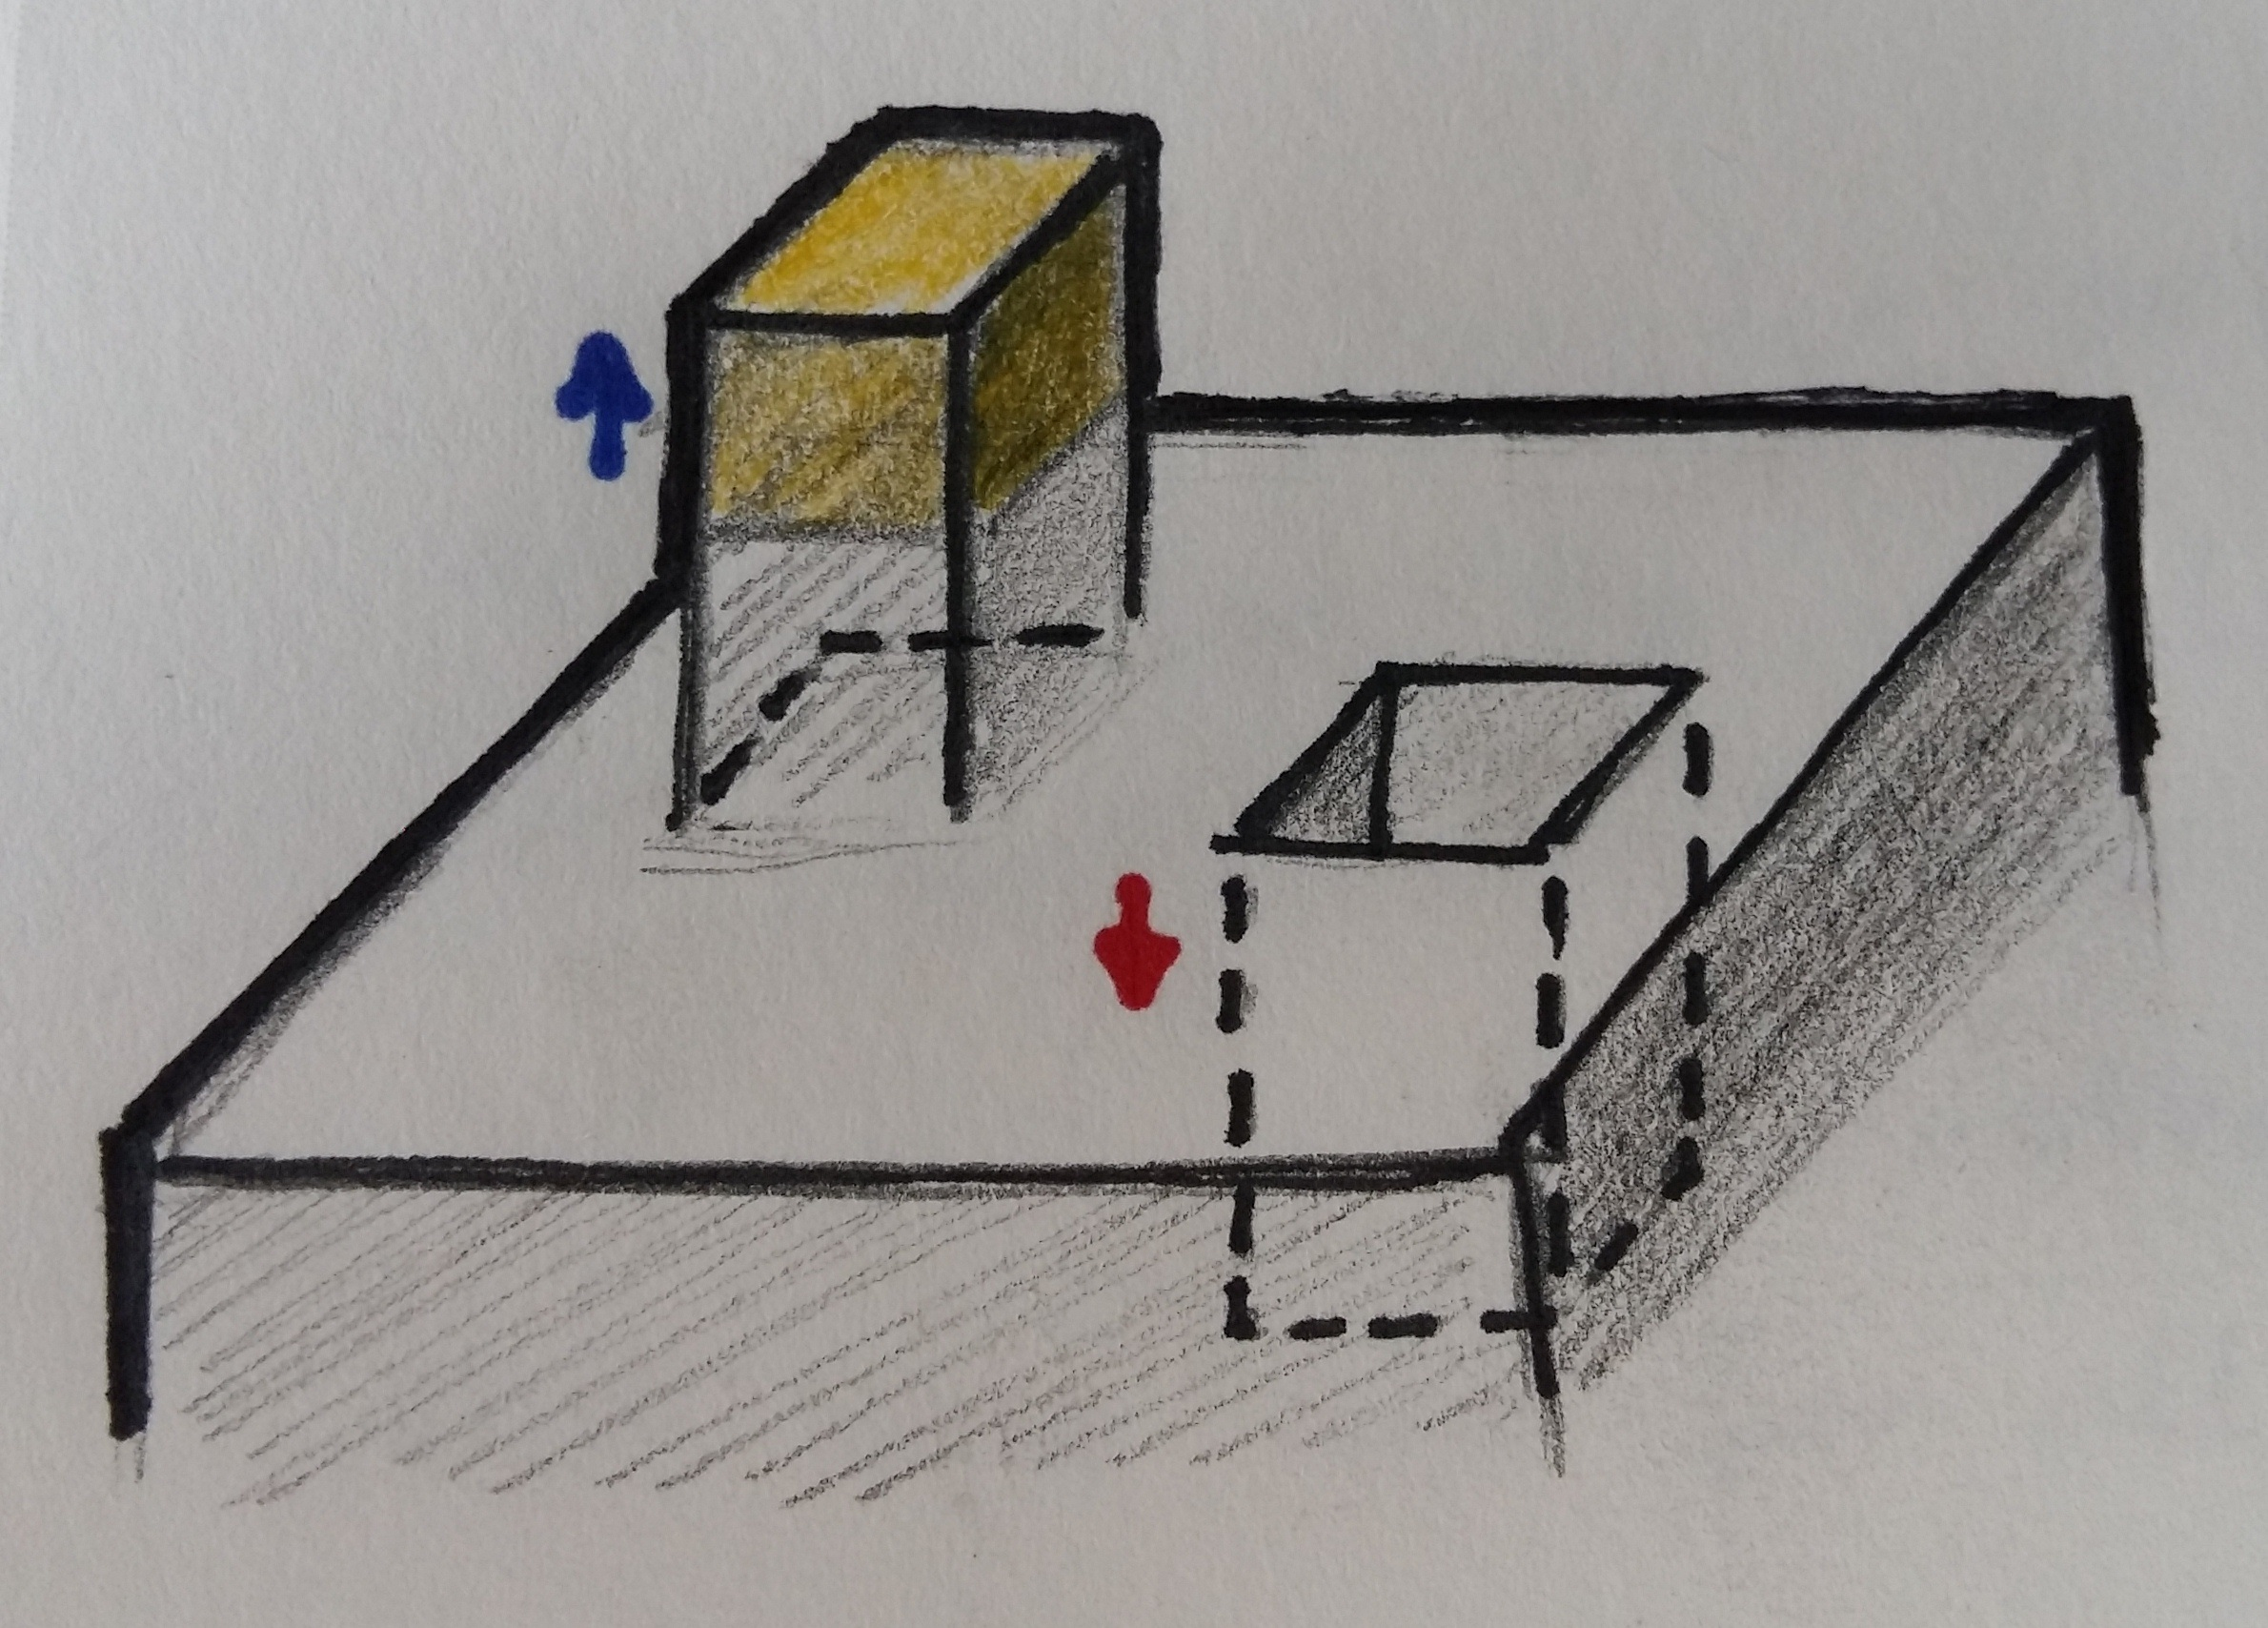
\includegraphics[width=0.5\textwidth]{draft1}
	\legend{\fonteAP}
	\label{fig:rascunho-torre-buraco}
\end{figure}

% ---
\section{Primeira iteração: prova de conceito}\label{sec-primeira-iteracao-prova-conceito}
% ---

Uma vez decidido o conceito a ser explorado, um pequeno protótipo foi proposto 
para dar ao grupo uma noção mais palpável de como esse jogo se pareceria, como 
seria controlá-lo, que dificuldades imprevistas apareceriam e quais as medidas 
que precisariam ser tomadas para suplantá-las. Este protótipo inicial tinha 
como objetivo tanto familiarizar o grupo às ferramentas e tecnologias 
escolhidas para a realização do trabalho quanto ajudar a nivelar de maneira 
mais concreta a complexidade de sua implementação.

O protótipo deveria se ater apenas a uma mecânica básica da especificação 
do conceito: controle da elevação do terreno. O jogador teria acesso direto ao 
jogo - sem passar por telas de menu ou tutoriais - no qual se depararia com 
uma grade tridimensional de 5x5x5 cubos de terra, os quais poderia elevar 
ou rebaixar livremente. Um exemplo desta prova de conceito está demonstrado na \autoref{fig:primeiro-screenshot-terra}.

\begin{figure}[h]
	\centering
	\caption{Prova de conceito do jogo}
	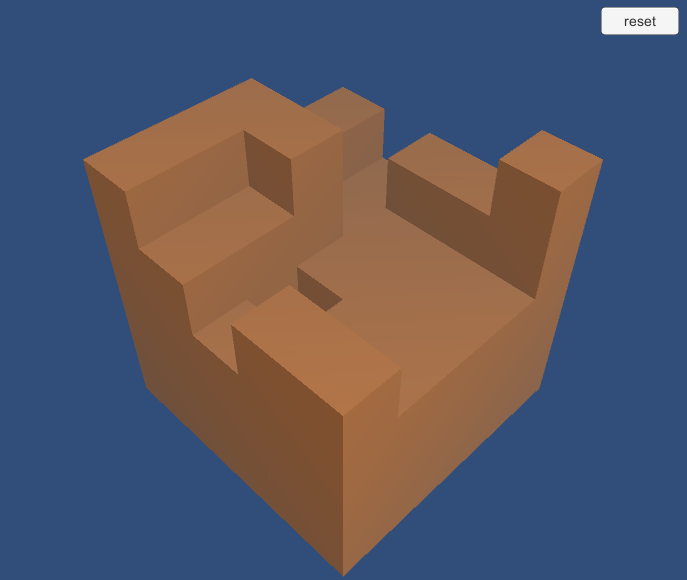
\includegraphics[width=0.5\textwidth]{ss1}
	\legend{\fonteAP}
	\label{fig:primeiro-screenshot-terra}
\end{figure}

Apesar da simples implementação, algumas primeiras dificuldades já puderam 
ser percebidas nesta iteração, sobretudo na integração dos dispositivos de 
realidade virtual.

A primeira barreira a ser percebida foi a falta de compatibilidade com 
dispositivos \textit{Android} da versão mais recente do \textit{SDK} do 
controlador \textit{Leap Motion}, como havia nas versões anteriores. Isso, aliado 
ao fato de que a versão anterior do \textit{SDK} não estava mais disponível 
para download, significou que uma interação direta entre o \textit{Leap Motion} 
e o jogo compilado para dispositivos móveis não seria possível nessa etapa 
inicial do projeto. A solução para este problema foi continuar o desenvolvimento
diretamente no computador, sem se preocupar em gerar a versão para o 
\textit{Android} (e, portanto, para o \textit{Google Cardboard}).

Apesar deste empecilho, \textit{Unity} se mostrou uma plataforma robusta e 
flexível o suficiente para a continuação do projeto, e as mecânicas básicas 
puderam ser implementadas rapidamente e sem grandes problemas.

% ---
\section{Segunda iteração: mecânicas básicas}\label{sec-segunda-iteracao-mecanicas-basicas}
% ---

Tendo em mente as facilidades e desafios percebidos durante a criação da prova 
de conceito, um segundo protótipo foi desenvolvido, desta vez com o intuito 
de acrescentar uma segunda mecânica básica - controle da precipitação - de modo
a permitir que o jogador experimentasse com a interação entre as duas.

Para tal, foi necessário especificar um pouco melhor a mecânica da água 
e como ela funcionaria em relação às mudanças de altura do terreno. 
Primeiro, definiu-se que a agua deveria crescer de baixo para cima, de
maneira similar a um recipiente sendo preenchido com líquido, demonstrado
na \autoref{fig:mecanica-agua-enchendo-graficamente}. Esta era uma
definição mais referente ao apelo gráfico do que uma mecânica. Adicionalmente, 
definiu-se que, dado um bloco (ou conjunto de blocos) selecionados, a ação de
precipitação preencheria o espaço aberto até cobrir os blocos selecionados, em 
vez de preencher de água para que esta fique no mesmo nível do bloco selecionado.
Esta mecânica pode ser vista na \autoref{fig:mecanica-agua-enchendo-mecanica}.

\begin{figure}[ht]
	\centering
	\caption{Mecânicas da água 1}
	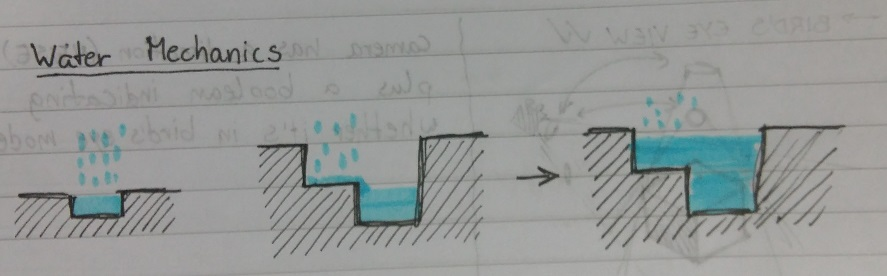
\includegraphics[width=0.5\textwidth]{water_mechanics1}
	\legend{\fonteAP}
	\label{fig:mecanica-agua-enchendo-graficamente}
\end{figure}

\begin{figure}[ht]
	\centering
	\caption{Mecânicas da água 2}
	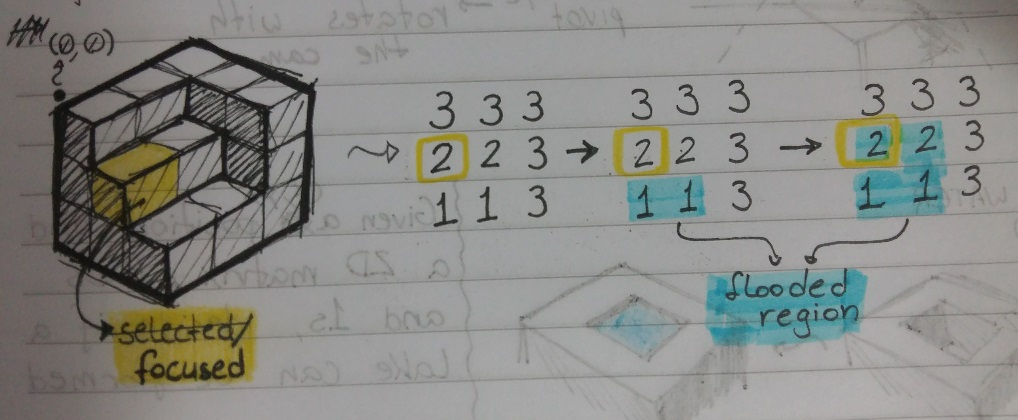
\includegraphics[width=0.5\textwidth]{water_mechanics2}
	\legend{\fonteAP}
	\label{fig:mecanica-agua-enchendo-mecanica}
\end{figure}

Nesta iteração, haveria dois gestos que deveriam ser captados e interpretados 
pelo \textit{Leap Motion}: abaixar e elevar a mão com a palma aberta para alterar 
a elevação do terreno e apontar todos os dedos para baixo para fazer chover em 
uma área específica.

Durante a implementação dessas mecânicas, ficou clara a necessidade de uma 
mecânica de seleção que permitisse a manipulação de grandes áreas do terreno
simultaneamente, então um terceiro gesto foi adicionado: pinçar e arrastar 
para delimitar áreas.

Também nessa etapa, percebeu-se que, devido à posição do \textit{Leap Motion},
alguns dos gestos imaginados para as diferentes mecânicas do jogo - sobretudo 
o associado a chuva - não poderiam ser captados com a precisão necessária, 
nos levando a precisar reimaginar uma parte significativa da interação. Isto 
resultou na simplificação do gesto para a chuva, bastante apenas fechar o punho
com a palma virada para baixo. Desta forma, o gesto era capturado mais facilmente,
mas também era ativado muitas vezes quando o jogador não havia feito o gesto, 
dificultando a jogabilidade. Uma possível razão para isto é ter definido o 
gesto de maneira não ótima, devido à inexperiência neste assunto por parte
dos integrantes do grupo.

Apesar de tudo, o protótipo já estava jogável e era possível modificar o terreno e adicionar ou remover água, como mostrado na \autoref{fig:example-water-earth}

\begin{figure}[ht]
	\centering
	\caption{Prova de conceito do jogo}
	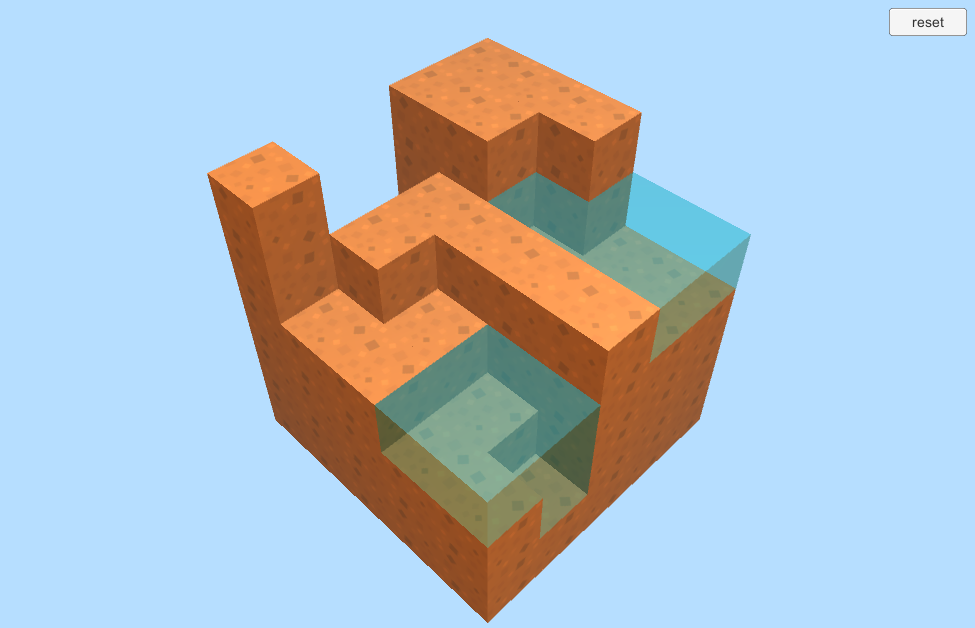
\includegraphics[width=0.5\textwidth]{ss2}
	\legend{\fonteAP}
	\label{fig:example-water-earth}
\end{figure}

% ---
\section{Terceira iteração: últimas mecânicas}\label{sec-terceira-iteracao-ultimas-mecanicas}
% ---

Ao final da segunda iteração, faltavam dois elementos para
completar o conjunto de elementos que o jogador poderia criar, de acordo
com o que havia sido definido: ar/vento e fogo.

O primeira é importante para ser possível criar fases que necessitem uma 
sequência maior de passos para se chegar ao objetivo e, portanto, criar
um desafio maior. Já o segundo é importante por sua reação com a água, 
que até então, quando criada, não podia ser removida. Desta forma, o 
fogo serve para desfazer movimentos errôneos de água. Dado a certa 
imprecisão existente com o gesto de geração de água, aonde o nosso
código acusava que o jogador havia feito o gesto erroneamente isto era
importante para minimizar a frustração do jogador.

% ---
\section{Quarta iteração: últimas mecânicas}\label{sec-quarta-iteracao-integracao}
% ---

Uma vez que os elementos principais foram implementados e o jogo já podia
ser jogado, focou-se em possibilitar a execução do jogo no android 
(que estava, até então, rodando no computador, por dificuldades 
discutidas na \autoref{sec-primeira-iteracao-prova-conceito}). Visto que
a primeira opção, que parecia a mais óbvia, não iria funcionar, foi feito um 
estudo mais a fundo sobre a arquitetura do sistema, que está descrita
na \autoref{sec-desenvolvimento-arquitetura}. 

Adicionalmente, correções foram feitas de bugs no código, e melhorias foram
feitas na detecção de gestos.

% ---
\section{Arquitetura}\label{sec-desenvolvimento-arquitetura}
% ---

Para se definir a arquitetura do sistema, é antes necessário identificar e 
entender cada um dos principais elementos, assim como suas interfaces.

% ---
\subsection{Identificação dos elementos}\label{subsec-identificacao-elementos}
% ---

% ---
\subsubsection{Controlador \textit{Leap Motion}}\label{subsubsec-elemento-leapmotion}
% ---

Conforme visto na Seção \ref{subsubsec-teo-leap-motion}, o controlador pode 
ser dividido em dois elementos diferentes: O \textbf{hardware do controlador} e 
o \textbf{serviço} que aplica algoritmos de visão computacional nas imagens 
vindas do hardware, transformando-as em dados estruturados.

O serviço pode ser executado no computador ou, no caso de se utilizar a versão 
v2 do \textit{SDK} do \textit{Leap Motion}, no \textit{Android}.

% ---
\subsubsection{Lógica do jogo}\label{subsubsec-elemento-logica-jogo}
% ---

Este é o elemento que age sobre o ambiente virtual a partir de dados de entrada 
do controlador e do movimento do \textit{headset} de realidade virtual. 
Este elemento estará implementado no Unity, e pode ser executado ou no 
computador ou no próprio celular.

% ---
\subsubsection{Processamento de saída do video}\label{subsubsec-elemento-video}
% ---

Este elemento é controlado pelo \textit{SDK} do \textit{Google Cardboard}, e 
cuida de toda a parte de gerar a visão estereoscópica necessária para a visão 
3D, além de movimentar a visão do jogo de acordo com o movimento do 
\textit{headset} de realidade virtual. Este elemento pode ser executado ou 
no computador ou no próprio celular.

% ---
\subsection{Arquiteturas estudadas}\label{subsec-arquiteturas-estudadas}
% ---

As três arquiteturas estudadas têm como entrada as imagens vindas do 
controlador \textit{Leap Motion} e do movimento do \textit{Google Cardboard}, 
que são enviadas à lógica de jogo que, então, modifica o estado do jogo e envia 
para o \textit{Google Cardboard}. As diferentes opções de arquitetura diferem 
quanto à como a conexão é feita, se é intermediada ou não por um computador, e 
aonde essa intermediação acontece.

% ---
\subsubsection{Alternativa utilizando o servidor WebSocket}\label{subsubsec-arquiteturas-leapmotion-pc-leapdata-android}
% ---

Nesta opção, conecta-se o controlador a um computador que esteja rodando o 
serviço do \textit{Leap Motion}, transformando as imagens do controlador em 
dados estruturados. O celular que está executando a lógica do jogo então se
conecta ao servidor \textit{websocket} gerado pelo serviço do controlador que 
esta rodando no computador. A partir desta conexão, o servidor envia os
dados estruturados ao celular para que estes possam ser utilizados como 
entradas no jogo. O celular então aplica as transformações necessárias para 
a saída de vídeo, que é enviada à tela do celular.
Esta opção é demonstrada na \autoref{fig:arquitetura-leap-pc-leapdata-android}.

As vantagens desta opção é que podemos utilizar a versão mais recente 
do \textit{SDK} do \textit{Leap Motion}, que melhorou muito o rastreamento das 
mãos, comparada à versão v2. Adicionalmente, o serviço já expõe uma interface 
web para a leitura dos dados estruturados. 

Uma desvantagen desta opção, porém, é a necessidade de modificar a biblioteca 
do \textit{Leap Motion} do \textit{Unity} para que esta aceite conexões web, já 
que, nativamente, ela aceita apenas conexões via USB. Outra desvantagem é a 
latência adicionada entre o movimento das mãos do usuário e o momento em que 
a lógica do jogo recebe tais informações. Se esta latência for alta demais, 
cria-se uma dissociação entre a mão do jogador e a mão virtual, diminuindo a imersão no jogo.

\begin{figure}[h]
	\centering
	\caption{Alternativa de arquitetura com servidor WebSocket}
	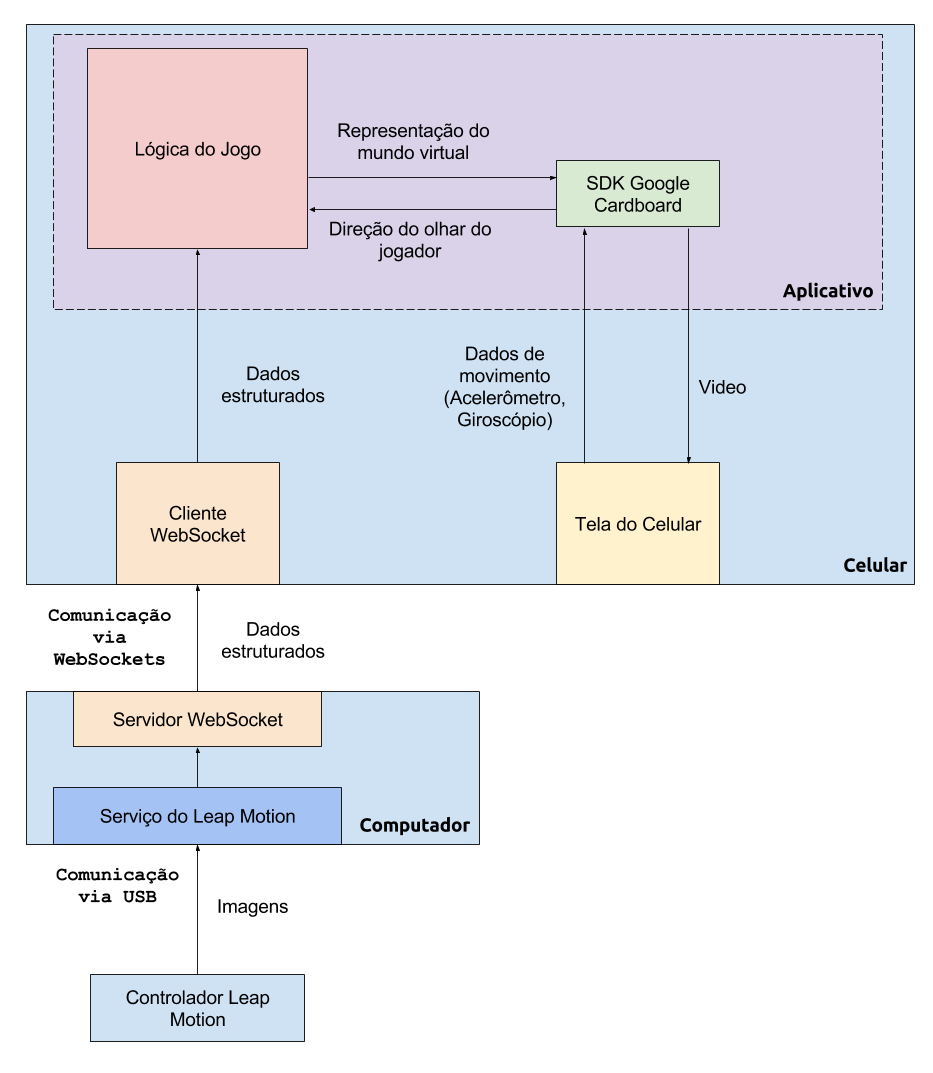
\includegraphics[width=0.7\linewidth]{images/Arquitetura-leap-pc-leapdata-android}
	\legend{\fonteAP}
	\label{fig:arquitetura-leap-pc-leapdata-android}
\end{figure}

% ---
\subsubsection{Alternativa com streaming do video}\label{subsubsec-arquiteturas-leapmotion-pc-riftcat-android}
% ---

O diferencial desta opção é que a lógica do jogo roda no computador, e a saída 
de vídeo é transmitida para o celular via algum software, como o Riftcat(pago) ou
o TrinusVR(gratuíto). Desta forma, o controlador é conectado diretamente 
ao computador, que está rodando o serviço do \textit{Leap Motion} e lê 
diretamente dele os dados estruturados. Esta arquitetura pode ser vista 
na \autoref{fig:Arquitetura-leap-pc-riftcat-android}.

As vantagens desta opção são que, por rodar num computador, o poder de 
processamento é mais alto e, portanto, existem mais possibilidades quanto
a algoritmos utilizados, mecânicas do jogo e processamento gráfico. A conexão 
com o controlador, por ser direta, também significa uma latência baixa 
neste quesito. 

O principal contraponto desta opção é o aumento da latência entre o movimento 
da cabeça do usuário e o movimento da cabeça virtual. Esta latência é maior do 
que a da primeira opção pois é necessário enviar os dados referentes ao movimento 
da cabeça do celular para o computador, que então deve enviar as imagens de 
volta para o celular. Essa latência adicional não apenas cria uma dissociação 
entre o jogador e o mundo virtual, mas também pode causar tontura e enjoo.

\begin{figure}
	\centering
	\caption{Alternativa de arquitetura com streaming do video}
	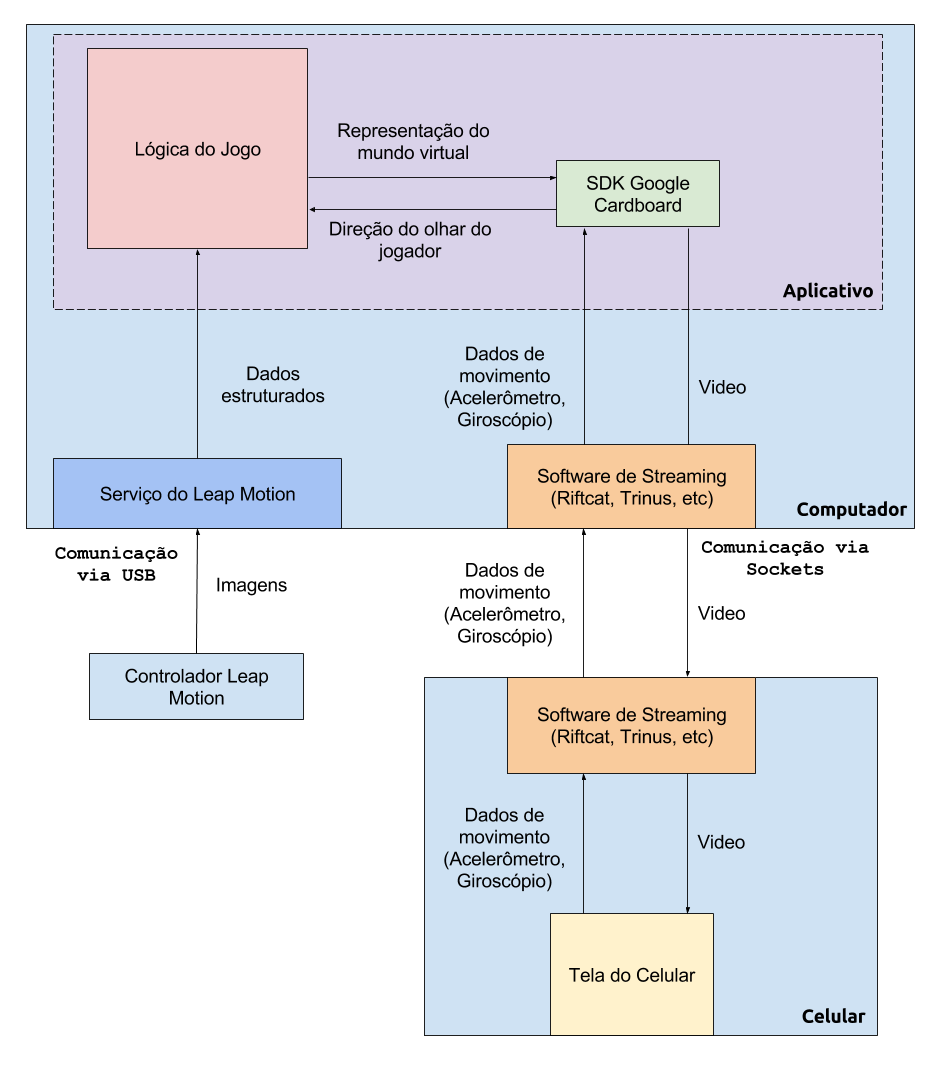
\includegraphics[width=0.7\linewidth]{images/Arquitetura-leap-pc-riftcat-android}
	\legend{\fonteAP}
	\label{fig:Arquitetura-leap-pc-riftcat-android}
\end{figure}

% ---
\subsubsection{Alternativa com conexão direta}\label{subsubsec-arquiteturas-leapmotion-android}
% ---

Nesta opção, o controlador é conectado diretamente ao celular, conforme 
mostrado na \autoref{fig:arquitetura-leap-android}. Desta forma, esta opção 
provê a maior mobilidade e tem o menor número de subsistemas diferente. Para 
tal, é necessário utilizar o serviço do \textit{Leap Motion} v2 específica para 
o \textit{Android}. Neste caso, todo o processamento é feito diretamente no 
celular (A transformação das imagens em dados estruturados; a lógica do jogo e 
as transformações necessárias para a saída de video). Por esta razão, esta é a 
opção que adiciona a menor latência, devido à inexistência de conexões extras 
entre um computador e o celular, como nas outras opções.

As desvantagens, porém, são a dependência do serviço do \textit{Leap} nativo 
do \textit{Android}, que estava na versão beta antes de ser descontinuado, e 
também o fato de se tratar da versão v2, que tem um rastreamento pior.

\begin{figure}
	\centering
	\caption{Alternativa de arquitetura com conexão direta}
	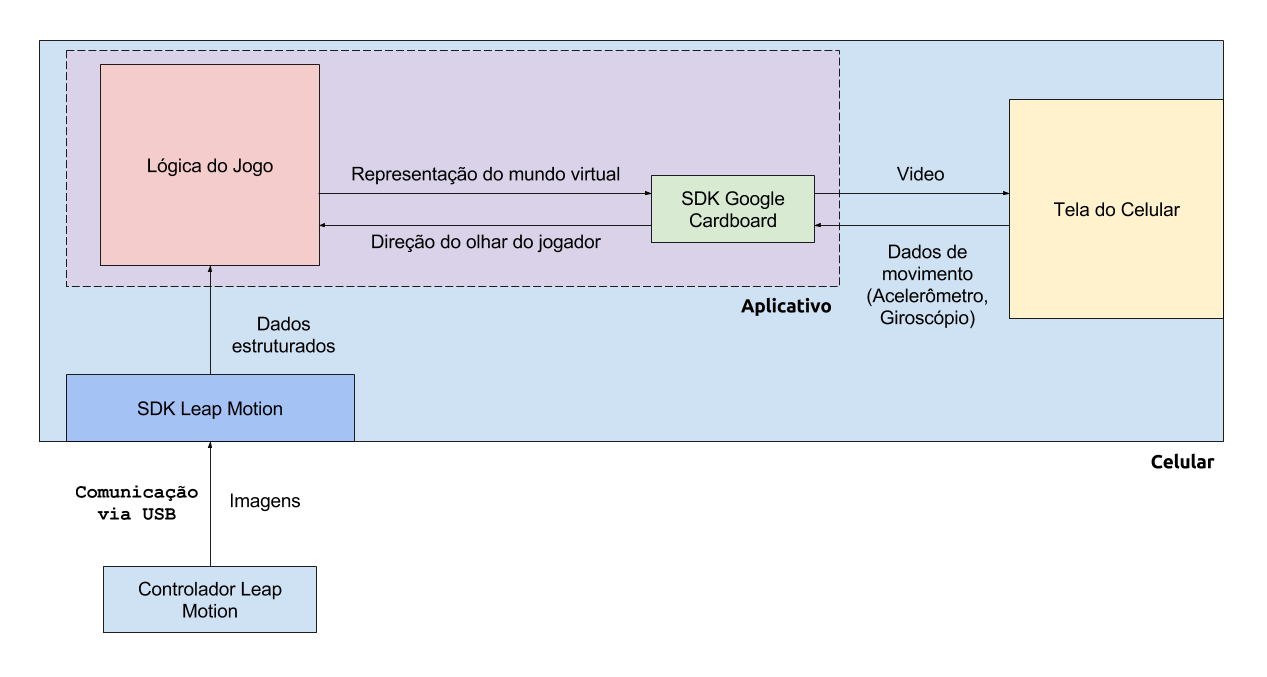
\includegraphics[width=0.7\linewidth]{images/Arquitetura-leap-android}
	\legend{\fonteAP}
	\label{fig:arquitetura-leap-android}
\end{figure}

% ---
\subsubsection{Comparação das alternativas}\label{subsubsec-arquiteturas-comparacao}
% ---

A comparação das alternativas pode ser vista no \autoref{tabela:alternativas-arquiteturas}.

\begin{quadro}[htb] \scriptsize
	\centering
	\caption[Comparação das alternativas de arquitetura]{Comparação das alternativas de arquitetura}
		
	\begin{tabular}{|>{\centering\arraybackslash}m{2.1cm}|>{\centering\arraybackslash}m{6cm}|>{\centering\arraybackslash}m{6cm}|}
		\hline 
		\textbf{Alternativa} & \textbf{Pros} & \textbf{Contras} \\
		\hline 
		Servidor Websocket
		&\begin{itemize}[label={},leftmargin=1mm]
			\item Versão mais recente do \textit{SDK} do \textit{Leap}.
			\item Servidor \textit{WebSocket} já disponível com o serviço \textit{Leap Motion}.
		\end{itemize}
		&\begin{itemize}[label={},leftmargin=1mm]
			\item Maior latência entre o movimento da mão e da mão do jogador, pode diminuir imersão.
			\item Necessidade de modificação da biblioteca do \textit{Leap} no \textit{Unity}.
		\end{itemize}
		\\ \hline 
		\textit{Streaming} de Video
		&\begin{itemize}[label={},leftmargin=1mm]
			\item Processamento feito no computador
			\item Conexão direta da lógica do jogo com controlador
		\end{itemize}
		&\begin{itemize}[label={},leftmargin=1mm]
			\item Latência entre movimento da cabeça do jogador e movimento da cabeça virtual, podendo causar desconforto e náusea.
			\item Dependência de mais software, podendo ser pago, e que pode ter como requisito um hardware mais caro para funcionar.
		\end{itemize}
	    \\ \hline 
		Conexão Direta
		&\begin{itemize}[label={},leftmargin=1mm]
				\item Menor latência dentre as opções
				\item Maior mobilidade
				\item Não depende de um computador
			\end{itemize}
		&\begin{itemize}[label={},leftmargin=1mm]
				\item Utiliza a versão v2 do \textit{SDK} do \textit{Leap}, que tem precisão pior.
				\item Necessita da versão beta do serviço para o \textit{Android}, de difícil acesso.
			\end{itemize}
		\\ 
		\hline 
	\end{tabular} 

	\legend{\fonteAP}
\label{tabela:alternativas-arquiteturas}
\end{quadro}

É possivel ver que as alternativas que não têm a conexão direta introduzem latências no sistema, mas em locais diferentes. O servidor \textit{Websocket} introduz latência na entrada referente ao movimento das mãos, enquanto o \textit{streaming} de video adiciona atrasos na saída do vídeo para o \textit{headset}. Por outro lado, a alternativa da conexão direta utiliza uma versão anterior do \textit{SDK} do controlador, que tem um rastreamento pior.

% ---
\subsection{Escolha da arquitetura}\label{subsec-arquitetura-escolha}
% ---

Inicialmente, havia se optado pela alternativa da conexão direta. Porém, devido
a impossibilidade de se utilizar a versão \textit{Orion} do \textit{SDK} do 
\textit{Leap Motion}, foi necessário mudar de alternativa. A alternativa 
escolhida foi a do \textit{streaming} de video, visto que a 
sua implementação não necessitaria de mudanças no código. Bastaria gerar 
o executável do jogo no Windows e rodar um software de \textit{streaming}, como o 
Riftcat. Esta alternativa foi testada por um tempo, aonde se constatou
alguns defeitos, como a necessidade de se reiniciar o software várias vezes 
devido a bugs e falta de documentação do Rifcat. Mesmo assim, devido a facilidade
de implementação e qualidade aceitável da solução, a alternativa foi escolhida
como a que seria utilizada.

Porém, descobriu-se posteriormente, ao se testar o software nos computadores
dos outros membros do grupo, que para que esta alternativa funcionasse, 
era necessário uma placa de video relativamente potente, de acordo com 
as especificações mínimas do software, encontrada em
\cite{riftcat:2016:requirements}. Inclusive, o software do Riftcat só 
funcionava em um dos cinco computadores testados. Por esta razão, optou-se 
por abandonar esta alternativa, visto que dificultaria a acessibilidade do jogo.

Dado este contratempo, decidiu-se verificar a viabilidade das outras duas 
alternativas. A alternativa da conexão direta havia sido descartada devido
à remoção do \textit{SDK} do site do \textit{Leap Motion}. 
Afortunadamente, a co-orientadora 
deste projeto havia trabalhado anteriormente com o \textit{Leap Motion} 
no \textit{Android}, e conseguiu uma cópia dos arquivos necessários. 
Entretanto, nos testes preliminares feitos, não se obteve sucesso na 
utilização do serviço: O aplicativo do software no celular reconhecia o 
controlador conectado, mas aplicativos 'clientes' que utilizariam os 
dados do controlador não conseguiam conectar-se ao controlador. Por este 
motivo, esta alternativa foi descartada.

Optou-se então pela alternativa que restou, que utiliza o servidor
\textit{WebSocket} gerado pelo serviço do \textit{Leap Motion} no computador. 
A principal dificuldade desta alternativa é que o plugin disponibilizado 
pela empresa para o \textit{Unity} só conseguia receber os dados do controlador 
por meio da conexão direta, e não pelo servidor \textit{WebSocket}. Portanto, foi 
necessário modificar o plugin distrubuído, que é software livre e tem seu 
código fonte disponível, para que ele se conectasse ao servidor \textit{WebSocket}, 
recebesse os dados estruturados em mensagens JSON, parseasse-as e 
então as transformasse na estrutura de dados utilizada pelo \textit{Unity}.

Para implementar tais mudanças no código do \textit{plugin}, foi necessário encontrar 
e testar bibliotecas que se conectassem a um servidor
\textit{WebSocket} (visto que o \textit{Unity} não consegue fazer 
isto nativamente) e parseasse JSON (pois o \textit{parser} JSON nativo 
do \textit{Unity} só funciona em casos de uso muito limitados). Visto que 
é necessário que movimentos das mãos sejam refletidos o mais rapidamente 
o possível no jogo (para se manter a impressão de que as mãos virtuais 
são as mãos reais do usuário, para manter a imersão), é essencial que 
estas bibliotecas fossem rápidas o suficiente para não serem um gargalo. 
Como, no \textit{Unity}, é o próprio \textit{framework}
que faz a gerência da sua memória (ou seja, o \textit{Unity} roda o coletor de 
lixo de tempos em tempos, em oposição ao programador ter de se preocupar com isto)
é necessário também que os algoritmos sejam eficientes em questão de memória 
e objetos alocados, visto que rodam com frequência alta e que a execução do
coletor de lixo pode causar travamentos dependendo de quantos objetos 'mortos' 
existirem.

Uma dificuldade encontrada nesta parte de modificação do \textit{plugin} é que o
\textit{Unity} tem um \textit{profiler} interno, que permite ver a alocação
de memória e dados sobre a performance do jogo, mas que só permite esse
monitoramento no \textit{thread} principal do \textit{Unity}. Visto que a 
modificação do \textit{plugin} inseria a necessidade de se ficar esperando uma 
mensagem chegar do servidor \textit{WebSocket}, e que fazer isto na 
\textit{thread} principal acarretaria em uma grande queda de desempenho, 
o código que recebe as mensagens do servidor e que as transforma nos dados
esperados pelo \textit{Unity} foi colocado para executar em uma \textit{thread}
secundária. Portanto, com o \textit{profiler} interno do \textit{Unity} não
era possivel se monitorar diretamente o desempenho da \textit{thread}, sendo 
necessário estimar o desempenho através das consequências dos resultados do 
\textit{thread} secundário, ou através da impressão do valor de variáveis
no console.


\TODO{Lucy: falta o capítulo com a pesquisa           }        
     
\TODO{Lucy: falta o capítulo com os resultados da pesquisa    }    
                
\TODO{Lucy: falta a conclusão                     }   

\TODO{Lucy: na introdução falta também os trabalhos relacionados. }       
               
\TODO{Lucy: em nenhum momento vocês falam onde está sendo
	 aplicado as habilidades no jogo de vocês.                        }
 
\TODO{Lucy: isso precisa ficar claro em algum lugar.}

\TODO{Lembrete: Apendice - Feito por nos. Anexo: Nao feito por nós.}

\TODO{Lembrete: Questionario foi validado, sim.}

% o \label{codigo} serve para podermos fazer referencias para algo numerado, 
% como capitulos, tabelas, figuras, etc. 
% Quando colocamos o comando \ref{codigo}. o compilador troca o \ref{codigo}
% pelo numero atribuido ao \label{}
% ex. \label{tabelaLegal}
%   A tabela \ref{tabelaLegal} mostra que...
% vai ser substituido por
%   A tabela 2 mostra que

\chapter{Considerações finais}\label{cap-consideracoes-finais}

O objetivo deste trabalho foi criar um jogo efetivamente educacional, capaz de manter o engajamento e interesse do jogador, de forma a ajudar a exercitar habilidades de raciocínio lógico, além de desenvolver uma solução final de baixo custo que possa ser implementada em instituições educacionais.

% ---
\section{Principais resultados}\label{sec-conc-resultados}
% ---

Foi desenvolvido um jogo digital, utilizando realidade virtual 
e o controle através das mãos, que entreteu os jogadores que o 
testaram, mesmo havendo algumas falhas no controlador. 

A solução também tem um custo acessível, se comparado a outras soluções 
de realidade virtual, devido ao uso de componentes de baixo custo e a 
possível reutilização de celulares \textit{smartphones} e \textit{laptops}. 
O jogo roda com latência aceitável, não necessita de um computador com 
componentes caros e de alto desempenho (como uma placa de video dedicada 
topo de linha), e é simples de configurar e executar.

Não foi possível aplicar o questionário criado, e portanto não foi 
possível obter dados qualitativos sobre o efeito do jogo sobre as 
competências e habilidades do raciocínio lógico. Porém, durante a 
sessão de \textit{playtesting} se constatou que os jogadores 
encaravam o jogo como um desafio lógico, comprovando em parte o 
exercício do raciocínio lógico.

% ---
\section{Contribuições}\label{sec-conc-contribuicoes}
% ---

As contribuições desse trabalho na nossa formação foram:

\begin{alineas}
	\item praticar o gerenciamento de projeto e o trabalho em grupo;
	\item criar uma visão do processo envolvido no desenvolvimento de um jogo do início ao fim;
	\item aprender novas tecnologias, como o controlador \textit{Leap Motion}, \textit{WebSockets} e o \textit{Google Cardboard};
	\item aplicar teorias aprendidas durante o curso.
\end{alineas}

Fatores que colaboraram para o projeto foram:

\begin{alineas}
	\item nossa co-orientadora, Profa. Msc. Lucy Mari Tabuti, ter conhecimento e experiência na área de jogos de lógica digitais, jogos educacionais, realidade virtual, e com o controlador \textit{Leap Motion};
	\item os integrantes do grupo ja terem um pouco de experiênca com o \textit{Unity}.
\end{alineas}

% ---
\section{Dificuldades}\label{sec-conc-dificuldades}
% ---

Em relação ao controlador \textit{Leap Motion}, houve dificuldade em detectar
movimentos específicos, tanto por inexperiência (conforme dito na
\autoref{sec-segunda-iteracao-mecanicas-basicas}) quanto por dificuldades 
em expressar os movimentos da forma correta, ao se tratar das relações entre 
os ossos e vetores que definiam a mão do jogador, conforme descrito na
\autoref{subsubsec-teo-gestos}.

Adicionalmente, houve dificuldade de se aplicar os testes em crianças pois
suas mãos, possivelmente pelo seu tamanho menor, não eram detectadas muito 
bem pelo controlador. Conforme descrito na 
\autoref{sec-roteiro-observacoes}, porém, é possível que este problema 
tenha sido devido à iluminação do local, que atrapalha o controlador.

A definição da arquitetura também encontrou obstáculos, visto que a 
primeira escolha de arquitetura teve de ser modificada devido 
a problemas relacionados ao hardware. Também ocorreu problemas devido à falta de documentação de elementos, como da versão \textit{Android} da biblioteca do \textit{Leap Motion} e do software \textit{Riftcat}.

% ---
\section{Trabalhos futuros}\label{sec-conc-trabalhos-futuros}
% ---

Dado que não foi possível aplicar o questionário com pessoas pertencentes ao 
público alvo, um próximo passo seria este. Desta forma, seria possível verificar 
o quão benéfico o jogo é.

Adicionalmente, novas fases com novas mecânicas podem ser implementadas no 
futuro, aumentando o tamanho do jogo, de forma a permitir que jogadores 
passem mais tempo se divertindo, enquanto exercitam suas habilidades de 
raciocínio lógico.

Melhorias no código, em especial no reconhecimento de gestos utilizados 
para ações também são um próximo passo importante, por tornar o jogo 
menos frustrante ao usuário, que não mais precisará repetidamente executar 
um mesmo gesto para tentar ativar uma ação.

%\label{part:planejamento}
%\input{chap/spec}

%\input{chap/tecno}

%\input{chap/met}

%\part{Aplicação}
%\label{part:aplicacao}
%\input{chap/imp}

%\input{chap/int}

% ---
% Finaliza a parte no bookmark do PDF, para que se inicie o bookmark na raiz
% ---
% TODO: Joao says: comentei a linha abaixo porque as seções do chap/concl apareciam como continuação
% do chap/int
% \bookmarksetup{startatroot}%
% ---

% ---
% Conclusão
% ---
%\input{chap/concl}



% ----------------------------------------------------------
% ELEMENTOS PÓS-TEXTUAIS
% ----------------------------------------------------------
\postextual


% ----------------------------------------------------------
% Referências bibliográficas
% ----------------------------------------------------------
\bibliography{references}

% ----------------------------------------------------------
% Glossário
% ----------------------------------------------------------
%
% Consulte o manual da classe abntex2 para orientações sobre o glossário.
%
%\glossary

% ----------------------------------------------------------
% Apêndices
% ----------------------------------------------------------


    % ---
    % Inicia os apêndices
    % ---
    \begin{apendicesenv}

        % Imprime uma página indicando o início dos apêndices
        \partapendices

		
\chapter{Experimento - Cubo de Gaia}
\noindent
\setlength{\parindent}{0pt}

\textbf{Perfil do sujeito de pesquisa}

Idade: \noindent\rule{1.5cm}{0.4pt} anos

Sexo: ( ) Masculino ( ) Feminino


\textbf{Experiência}

\textit{Selecione a alternativa mais adequada sobre a experiência geral do jogo}

1 – A experiência foi divertida

Discordo plenamente ( ) 1 ( ) 2 ( ) 3 ( ) 4 ( ) 5 ( ) 6 ( ) 7 Concordo plenamente



2 – A experiência foi desafiadora

Discordo plenamente ( ) 1 ( ) 2 ( ) 3 ( ) 4 ( ) 5 ( ) 6 ( ) 7 Concordo plenamente


3 – A experiência foi educativa

Discordo plenamente ( ) 1 ( ) 2 ( ) 3 ( ) 4 ( ) 5 ( ) 6 ( ) 7 Concordo plenamente


4 – A experiência foi injusta em um ou mais momentos

Discordo plenamente ( ) 1 ( ) 2 ( ) 3 ( ) 4 ( ) 5 ( ) 6 ( ) 7 Concordo plenamente

se sim, em que situação ou situações?

\rule{\linewidth-\marginparwidth}{0.4pt}


\textbf{Interface}

\textit{Selecione a alternativa mais adequada sobre os controles e estética do jogo}


5 – Os controles do jogo foram fáceis de compreender

Discordo plenamente ( ) 1 ( ) 2 ( ) 3 ( ) 4 ( ) 5 ( ) 6 ( ) 7 Concordo plenamente


6 – Os controles do jogo funcionaram corretamente

Discordo plenamente ( ) 1 ( ) 2 ( ) 3 ( ) 4 ( ) 5 ( ) 6 ( ) 7 Concordo plenamente


7 – O jogo funcionou bem com sensores de movimento

Discordo plenamente ( ) 1 ( ) 2 ( ) 3 ( ) 4 ( ) 5 ( ) 6 ( ) 7 Concordo plenamente


8 – Os gráficos e sons foram agradáveis

Discordo plenamente ( ) 1 ( ) 2 ( ) 3 ( ) 4 ( ) 5 ( ) 6 ( ) 7 Concordo plenamente



9 – Houve confusão para diferenciar os elementos do jogo

Discordo plenamente ( ) 1 ( ) 2 ( ) 3 ( ) 4 ( ) 5 ( ) 6 ( ) 7 Concordo plenamente

\textbf{Desafios}

\textit{Selecione a alternativa mais adequada sobre a resolução de fases individuais}


10 – O jogo funcionou bem com sensores de movimento

Discordo plenamente ( ) 1 ( ) 2 ( ) 3 ( ) 4 ( ) 5 ( ) 6 ( ) 7 Concordo plenamente



11 – A dificuldade entre as fases aumentou de forma justa

Discordo plenamente ( ) 1 ( ) 2 ( ) 3 ( ) 4 ( ) 5 ( ) 6 ( ) 7 Concordo plenamente



12 – Conhecimentos obtidos em fases anteriores se mostraram úteis na resolução das fases seguintes

Discordo plenamente ( ) 1 ( ) 2 ( ) 3 ( ) 4 ( ) 5 ( ) 6 ( ) 7 Concordo plenamente



13 – O objetivo apresentado nas fases ficou claro

Discordo plenamente ( ) 1 ( ) 2 ( ) 3 ( ) 4 ( ) 5 ( ) 6 ( ) 7 Concordo plenamente

se não, em que situação? 

\rule{\linewidth-\marginparwidth}{0.4pt}


\textbf{Comentários}

Comentários, críticas ou sugestões?

\rule{\linewidth-\marginparwidth}{0.4pt}

\rule{\linewidth-\marginparwidth}{0.4pt}

\rule{\linewidth-\marginparwidth}{0.4pt}

    \end{apendicesenv}

% ---


% ----------------------------------------------------------
% Anexos
% ----------------------------------------------------------
% ---
% Inicia os anexos
% ---
\begin{anexosenv}

% Imprime uma página indicando o início dos anexos
\partanexos

%\input{chap/comandosELM}

%\input{chap/pesquisa}

\end{anexosenv}


%---------------------------------------------------------------------
% INDICE REMISSIVO
%---------------------------------------------------------------------

\begin{comment}
\printindex
\end{comment}

\end{document}
